% Autor: Jose Ricardo Bustos Molina
%        Universidad del Tolima
%        jrbustosm@ut.edu.co
%

\chapter{Manual de usuario CALINA}

CALINA es una aplicación para móviles que tengan el sistema operativo Android \faAndroid, su propósito 
principal de brindarle a profesores una herramienta que medie técnicas de gamificación en el
desarrollo normal de su guía de aprendizaje. Por lo que CALINA, no es un juego como tal, es una estrategia 
pedagógica que complementa las clases, enriqueciéndose mediante el uso de mecánicas propia de los videojuegos 
\faGamepad\ y de los juegos de Rol \faShield.

Es bajo esta filosofía en la que es la aplicación la que se debe adaptar y complementar a tu clase, y no al 
contrario que tu clase se debe adaptar a la herramienta existente, que CALINA fue desarrollada, por lo que 
podrás asignar puntos para dar la sensación de progreso \faStarO, dar el poder a tus alumnos que sus acciones 
valgan en la vida real, desarrollen una historia que complemente el aprendizaje, cooperen entre ellos 
\faUsers, les puedas premiar al momento \faGift\ y ellos sean recompensados con objetos concretos por sus 
logros \faTrophy, ...., bueno y muchas cosas mas, que están por crearse en el mundo de CALINA, acá podrás 
hacer juegos de \textit{scape room} en el mundo real, carreras de observación \faMap, cursos de escritura 
colaborativa, y muchos estrategias mas, que tu imaginación es el límite y CALINA te ayuda a llegar allá.

Solo, para iniciar, que tal una aplicación que premie a tus estudiantes solo por asistir, pues con CALINA es 
posible, vamos a aprender a usarlo \faHeart:

\section{Requerimientos mínimos}

A pesar de la limitación inicial con la que se creo CALINA, pensando en los estudiantes y colegios que no 
tienen acceso a Internet, se decidió desde el inicio del diseño que todas las formas de transferencia de 
información debían realizarse sin usar los datos. Por lo que CALINA no requiere tener acceso a datos, y se 
opto por el uso de códigos QR \faQrcode\ por su versatilidad para realizar dicha transferencia y posibilidad 
de usar elementos impresos en clase, con las limitaciones de tamaño que conlleva, por lo tanto no se requiere 
el uso de los datos pero si tener permisos en el uso de la cámara \faCamera.

\begin{itemize}
	\item \textbf{Sistema Operativo:} mínimo Android 8.0 (nivel de API 26)
	\item \textbf{Permisos:} permiso de cámara, permiso de escritura memoria interna/externa
	\item \textbf{Espacio de memoria:} mínimo \qty{50}{\mega\byte}
	\item \textbf{Cámara:} cámara en funcionamiento
\end{itemize}

\section{Interfaz gráfica}

La interfaz principal de CALINA esta compuesta por 5 zonas, inicialmente se pertenece al grupo "CALINA" y 
viene cargado con tarjetas de este grupo como misión de entrenamiento, sin embargo la configuración de las 
zonas puede variar dependiendo si tenemos el rol de estudiante o de profesor, esto es de acuerdo al contexto 
del grupo que tengamos seleccionado.

Como ya se mencionó inicialmente se pertenece al grupo "CALINA", y de este grupo no se puede salir nunca, 
adicionalmente para este grupo siempre se tendrá el rol de estudiante, por lo que al momento de entrar por 
primera vez no se pueden crear cartas, para crear un grupo y cartas si deseas tener el rol de profesor, ver la 
sección \ref{sec:app_creacioncartas}, que trata el tema de creación de cartas.

%Se usa caption con opción vacía para que no aparezca en el TOC
\begin{figure}[!htb]
\caption[]{Aplicación CALINA, pantalla principal}
\centering
\begin{adjustbox}{width=15cm}
\begin{tikzpicture}
	\node[inner sep=0pt] at (0cm,0cm) {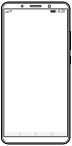
\includegraphics[width=7cm]{screenshots/movil}};
	\node[inner sep=0pt] at (-0.05cm,0.05cm) {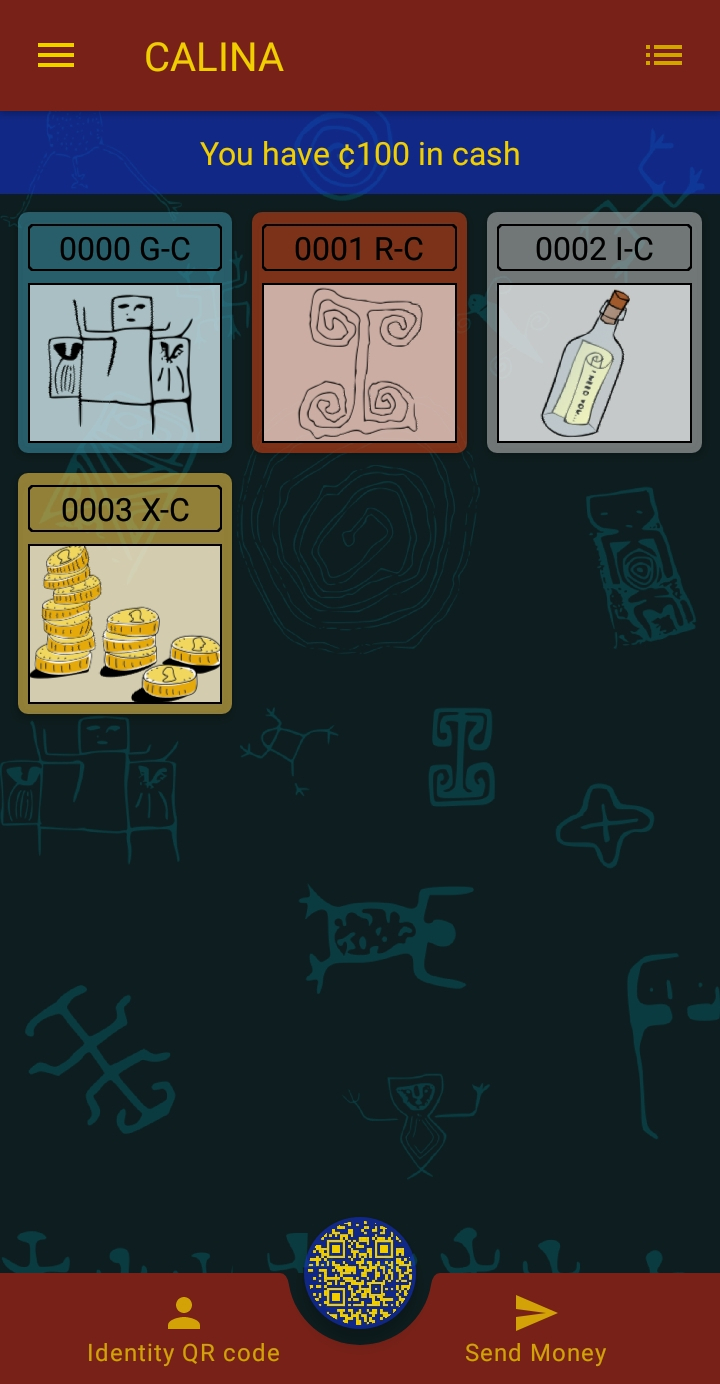
\includegraphics[width=5.95cm]{screenshots/pantalla_principal}};
	\draw[red, line width=0.4mm] (-2.85cm, 5cm) rectangle (-2.25cm, 5.65cm) {};
	\draw[red, line width=0.4mm] (-4cm, 5.32cm) -- (-2.85cm, 5.32cm);
	\node[red, anchor=east] at (-4.05cm, 5.32cm) {\textlangle A\textrangle\ Menú de navegación de grupos};
	\draw[cyan, line width=0.4mm] (2.2cm, 5cm) rectangle (2.75cm, 5.65cm) {};
	\draw[cyan, line width=0.4mm] (2.75cm, 5.32cm) -- (4cm, 5.32cm);
	\node[cyan, anchor=west] at (4.05cm, 5.32cm) {\textlangle B\textrangle\ Menú de filtro};
	\draw[magenta, line width=0.4mm] (-2cm, 5cm) rectangle (1.6cm, 5.65cm) {};
	\draw[magenta, line width=0.4mm] (-0.2cm, 5.65cm) -- (-0.2cm, 7.5cm);
	\node[magenta, anchor=south] at (-0.2cm, 7.5cm) {\textlangle C\textrangle\ Indicador grupo actual};
	\draw[green, line width=0.4mm] (-2.85cm, 4.2cm) rectangle (2.75cm, 4.85cm) {};
	\draw[green, line width=0.4mm] (-4cm, 4.52cm) -- (-2.85cm, 4.52cm);
	\node[green, anchor=east] at (-4.05cm, 4.52cm) {\textlangle D\textrangle\ Indicador de divisa / Rol};
	\draw[orange, line width=0.4mm] (-3.05cm, -3.9cm) rectangle (2.95cm, 4.1cm) {};
	\draw[orange, line width=0.4mm] (-4cm, 0.05cm) -- (-3.05cm, 0.05cm);
	\node[orange, anchor=east] at (-4.05cm, 0.05cm) {\textlangle E\textrangle\ Zona de las cartas};
	\draw[blue, line width=0.4mm] (-3.05cm, -5.65cm) rectangle (2.95cm, -4.1cm) {};
	\draw[blue, line width=0.4mm] (-4cm, -4.8cm) -- (-3.05cm, -4.8cm);
	\node[blue, anchor=east] at (-4.05cm, -4.8cm) {\textlangle F\textrangle\ Zona de controles};
\end{tikzpicture}
\end{adjustbox}
\\
{\footnotesize Fuente: de elaboración propia}
\end{figure}

A continuación se describe en detalle cada zona de la interfaz gráfica.

\subsection{Menú de navegación de grupos}

\begin{figure}[!htb]
\caption[]{Aplicación CALINA, menú de navegación de grupos}
\centering
\begin{adjustbox}{width=5cm}
\begin{tikzpicture}
	\node[inner sep=0pt] at (0cm,0cm) {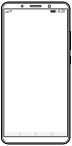
\includegraphics[width=7cm]{screenshots/movil}};
	\node[inner sep=0pt] at (-0.05cm,0.05cm) {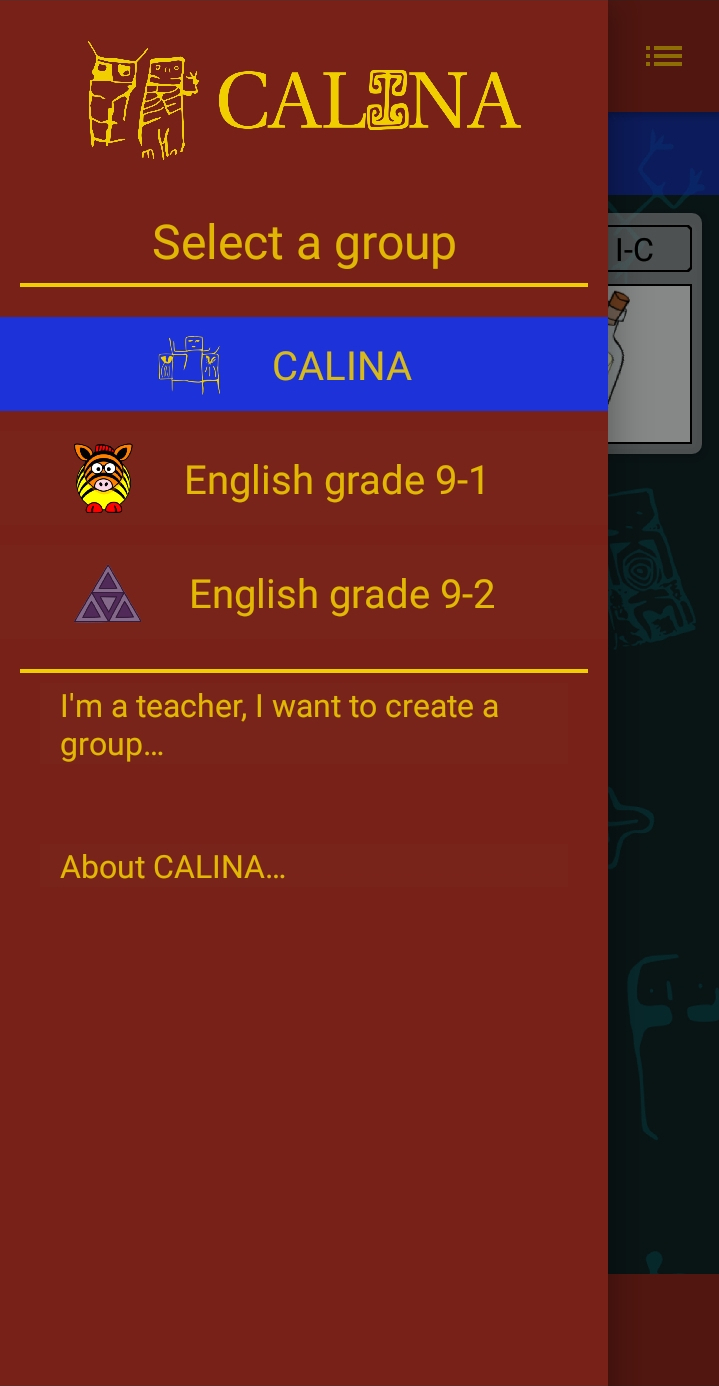
\includegraphics[width=5.95cm]{screenshots/menu_navegacion}};
\end{tikzpicture}
\end{adjustbox}
\\
{\footnotesize Fuente: de elaboración propia}
\end{figure}

Al hacer un toque sobre el icono de menú \faBars\ se desplaza desde la izquierda el menú lateral para la 
selección de grupos, cada grupo al que estemos registrados va a aparecer entre las dos lineas horizontales de 
este menú, el  grupo que actualmente tengamos seleccionado aparece resaltado con un rectángulo de color azul 
para resaltarlo del resto de grupos, y cada grupo tiene a su izquierda un icono o imagen que esta relacionado 
a la tarjeta de dicho grupo.

Otros elementos de este menú son, en la parte superior aparece el titulo e icono de la aplicación CALINA, y en 
la parte de abajo la opción de crear un grupo por si somos docentes y deseamos crear nuestro contexto de 
cartas para gamificar nuestra clase, así como la opción de ver un diálogo sobre créditos de la aplicación 
CALINA o cambiar el idioma de la aplicación.

\subsection{Menú de filtro}

\begin{figure}[!htb]
\caption[]{Aplicación CALINA, menú de filtros de cartas}
\centering
\begin{adjustbox}{width=5cm}
	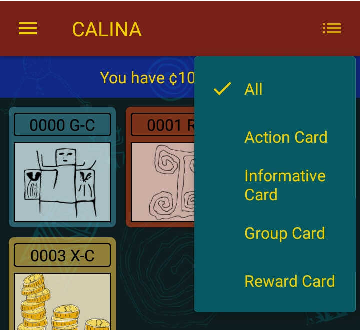
\includegraphics{screenshots/menu_filtro}
\end{adjustbox}
\\
{\footnotesize Fuente: de elaboración propia}
\end{figure}

Al hacer un toque en el icono de filtro \faList\ se desplaza un menú contextual abajo del icono, que permite
filtrar el conjunto de cartas del grupo seleccionado por tipo, las posibles opciones son cartas de 
información, de grupo, de acción, de recompensa y todas.

\subsection{Indicador grupo actual}

En esta sección, aparece el nombre del grupo que actualmente tengamos seleccionado, se modifica cada vez que 
cambiemos de grupo.

\subsection{Indicador de divisa / Rol}

\begin{figure}[!htb]
\caption[]{Aplicación CALINA, zona de divisas o indicador de rol}
\centering
\subfloat[Con rol de estudiante]{
	\begin{adjustbox}{width=7cm}
		
\includegraphics{screenshots/divisas}
	\end{adjustbox}
}
\hfill
\subfloat[Con rol de profesor]{
	\begin{adjustbox}{width=7cm}
		
\includegraphics{screenshots/rolprofesor}
	\end{adjustbox}
}
\\
{\footnotesize Fuente: de elaboración propia}
\end{figure}

Esta sección cambia de acuerdo al contexto, si somos estudiantes aparece la cantidad de divisa virtual que 
tengamos para el respectivo grupo, es importante aclarar que cada grupo cuenta con su propia moneda y el 
símbolo puede variar de grupo a grupo. Por otro lado, si somos propietarios del grupo, en otras palabras somos 
profesores, en esta zona se nos indica que tenemos este rol.

\subsection{Zona de las cartas}

Esta es la zona central de la aplicación CALINA, es donde aparecen las cartas que poseamos, y se mostraran las 
cartas de acuerdo al contexto que tengamos, es decir al grupo que pertenezcamos y el tipo de carta que 
tengamos marcado en el filtro de cartas, cada carta podemos hacerle un toque para ver en detalle su contenido 
y las posibles acciones que podemos ejecutar sobre ella.

Cada carta tiene un color característico de acuerdo al tipo de carta al que pertenece, y una información 
básica en la parte superior, que consta de un número de carta, su tipo y la dificultad de consecución.

\subsection{Zona de controles}

\begin{figure}[!htb]
\caption[]{Aplicación CALINA, zona de controles}
\centering
\subfloat[Con rol de estudiante]{
	\begin{adjustbox}{width=7cm}
		
\includegraphics{screenshots/controlesestudiantes}
	\end{adjustbox}
}
\hfill
\subfloat[Con rol de profesor]{
	\begin{adjustbox}{width=7cm}
		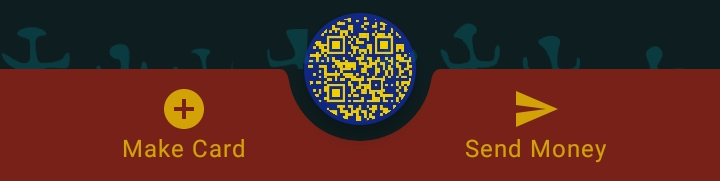
\includegraphics{screenshots/controlesprofesor}
	\end{adjustbox}
}
\\
{\footnotesize Fuente: de elaboración propia}
\end{figure}

Esta zona cambia de acuerdo al rol que tengamos, así es con el rol estudiante podemos generar un código de 
identificación QR que nos permite transmitir nuestra identidad única a otros celulares, un botón central para 
poder leer códigos QR, permitiendo recibir cartas nuevas o dinero virtual, y por último la posibilidad de 
enviar dinero a otras personas que pertenezcan al mismo grupo que nosotros.

Si tenemos el rol de profesor, tenemos en lugar de la posibilidad de generar un código de identificación, la 
opción de crear cartas para nuestros estudiantes.

\section{Tipos de cartas}

En la aplicación CALINA existen 4 tipos de carta, cada una con una función especifica, las \uline{cartas de 
agrupación} que permite identificar al estudiante a un grupo particular, las \uline{cartas de información} en 
la que se puede almacenar un texto, las \uline{cartas de recompensa} cuyo propósito es mostrar un logro del 
estudiante, y finalmente las \uline{cartas de acción} para permitir a los estudiantes generar acciones en la 
vida real.

\subsection{Cartas de agrupación (G)}

\begin{figure}[!htb]
\caption[]{Aplicación CALINA, cartas de agrupación}
\centering
\subfloat[Miniatura de carta de agrupación]{
	\begin{adjustbox}{width=2cm}
		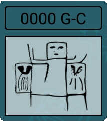
\includegraphics{screenshots/cartaagrupacion}
	\end{adjustbox}
}
\hspace{2cm}
\subfloat[Detalle de carta de agrupación]{
	\begin{adjustbox}{width=4cm}
		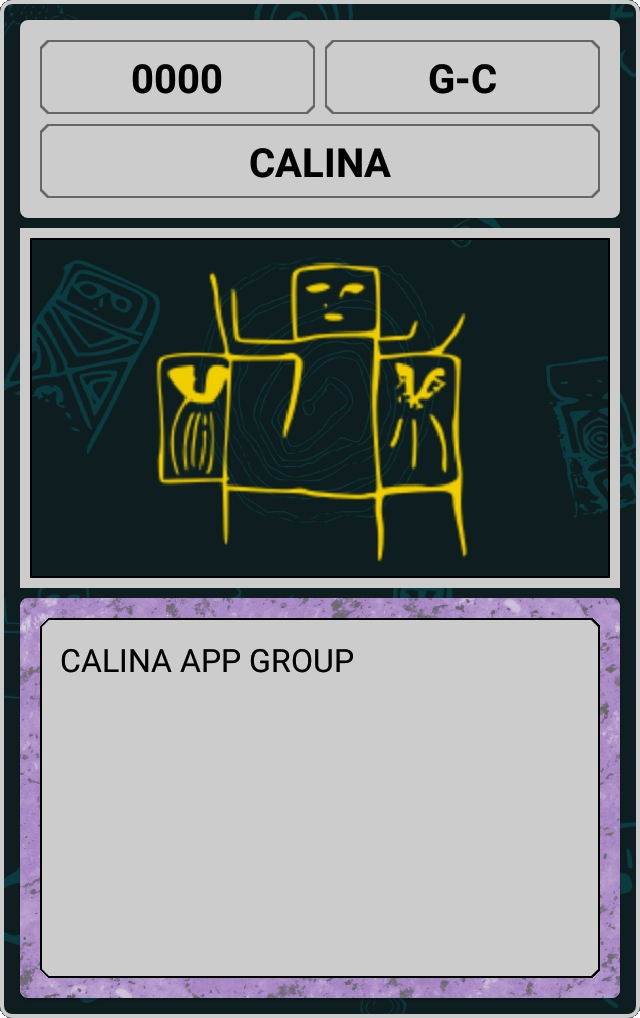
\includegraphics{screenshots/cartaagrupaciondetalle}
	\end{adjustbox}
}
\\
{\footnotesize Fuente: de elaboración propia}
\end{figure}

Identificadas con la letra \textbf{G}, las cartas de agrupación permiten que el estudiante pertenezca a un 
grupo en particular, creando en él sentimientos de pertenencia a un equipo, hay dos tipos de agrupaciones, los 
\uline{grupos principales:} que están asociados a una clase, este tipo de grupos es el que se selecciona en el 
respectivo menú de selección de grupos, por lo que siempre se debe poseer al menos una de estas cartas y al 
borrarla se deja de pertenecer a la clase en particular. Por otro lado, los \uline{grupos secundarios}, los 
cuales son cartas que permiten a un estudiante pertenecer a un grupo particular dentro de la propia clase.

\subsection{Cartas de información (I)}

\begin{figure}[!htb]
\caption[]{Aplicación CALINA, cartas de informacion}
\centering
\subfloat[Miniatura de carta de agrupación]{
	\begin{adjustbox}{width=2cm}
		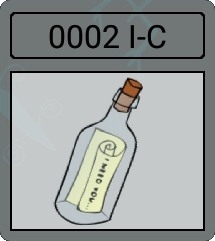
\includegraphics{screenshots/cartainformacion}
	\end{adjustbox}
}
\hspace{2cm}
\subfloat[Detalle de carta de agrupación]{
	\begin{adjustbox}{width=4cm}
		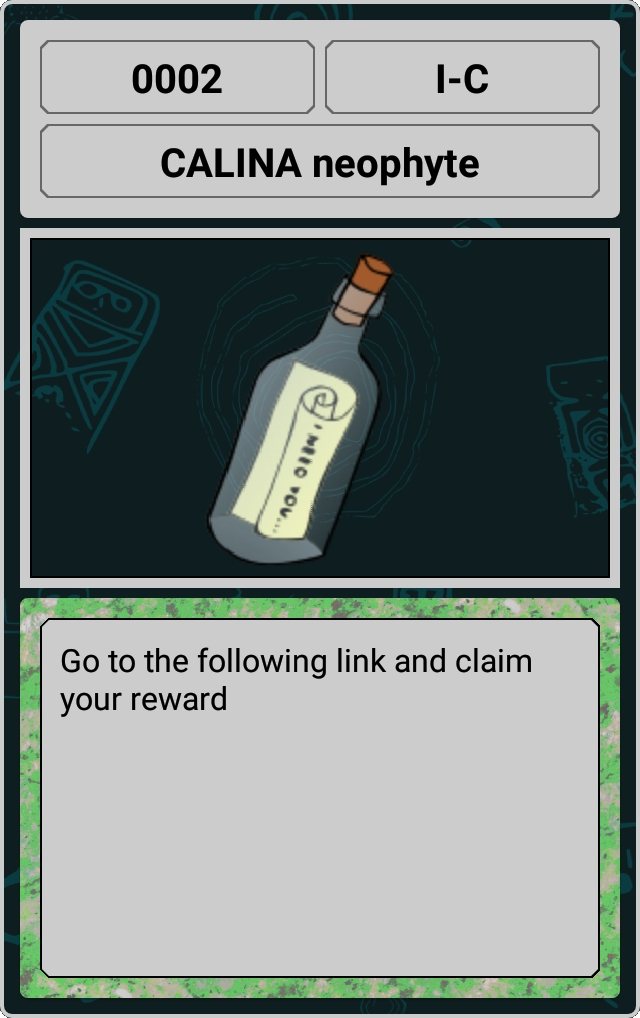
\includegraphics{screenshots/cartainformaciondetalle}
	\end{adjustbox}
}
\\
{\footnotesize Fuente: de elaboración propia}
\end{figure}

Identificadas con la letra \textbf{I}, las cartas de información permiten transmitir retos, historias, datos,
pistas, etc. a través del sistema de cartas de CALINA, existe la opción de poner \textit{links} junto con el 
texto para re-direccionar a información adicional en la web que amplíen la narrativa.

Adicional pueden existir cartas con la opción de editable, donde los estudiantes pueden modificar el texto de 
las cartas y así, mandar mensajes o contar historias cuando estas cartas son transferidas a otros miembros del 
grupo (incluido el docente propietario del grupo).

\subsection{Cartas de recompensa (R)}

Identificadas con la letra \textbf{R}, las cartas de recompensa permiten indicar el obtención de un logro por 
parte del estudiante.

\begin{figure}[!htb]
\caption[]{Aplicación CALINA, cartas de recompensa}
\centering
\subfloat[Miniatura de carta de agrupación]{
	\begin{adjustbox}{width=2cm}
		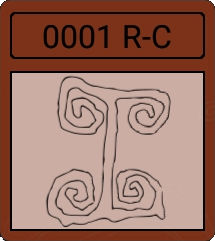
\includegraphics{screenshots/cartarecompensa}
	\end{adjustbox}
}
\hspace{2cm}
\subfloat[Detalle de carta de agrupación]{
	\begin{adjustbox}{width=4cm}
		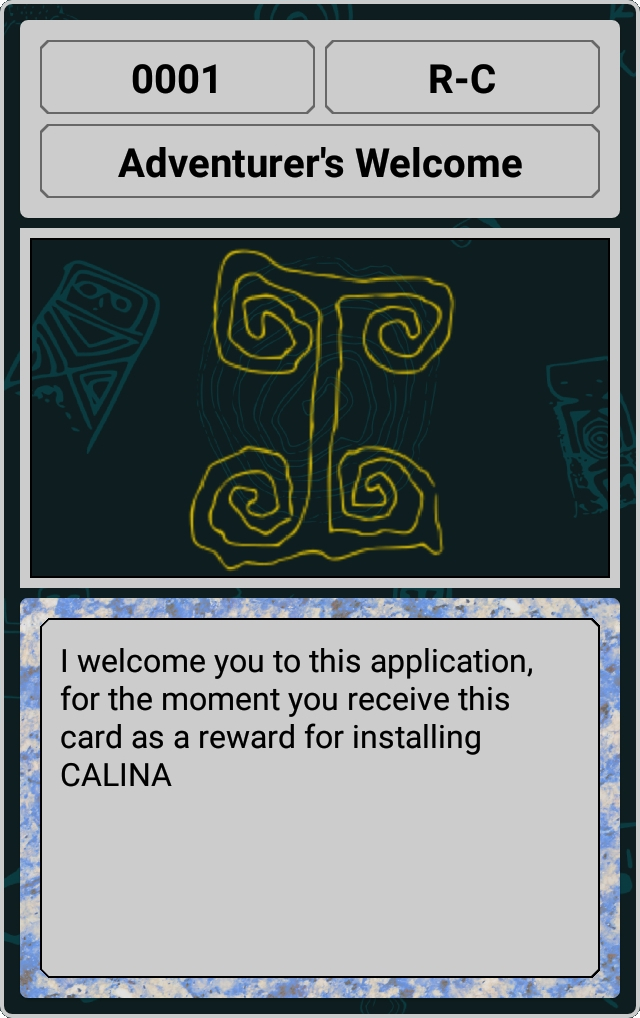
\includegraphics{screenshots/cartarecompensadetalle}
	\end{adjustbox}
}
\\
{\footnotesize Fuente: de elaboración propia}
\end{figure}

\subsection{Cartas de acción (X)}

\begin{figure}[!htb]
\caption[]{Aplicación CALINA, cartas de acción}
\centering
\subfloat[Miniatura de carta de agrupación]{
	\begin{adjustbox}{width=2cm}
		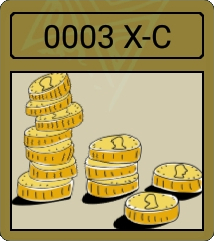
\includegraphics{screenshots/cartaaccion}
	\end{adjustbox}
}
\hspace{2cm}
\subfloat[Detalle de carta de agrupación]{
	\begin{adjustbox}{width=4cm}
		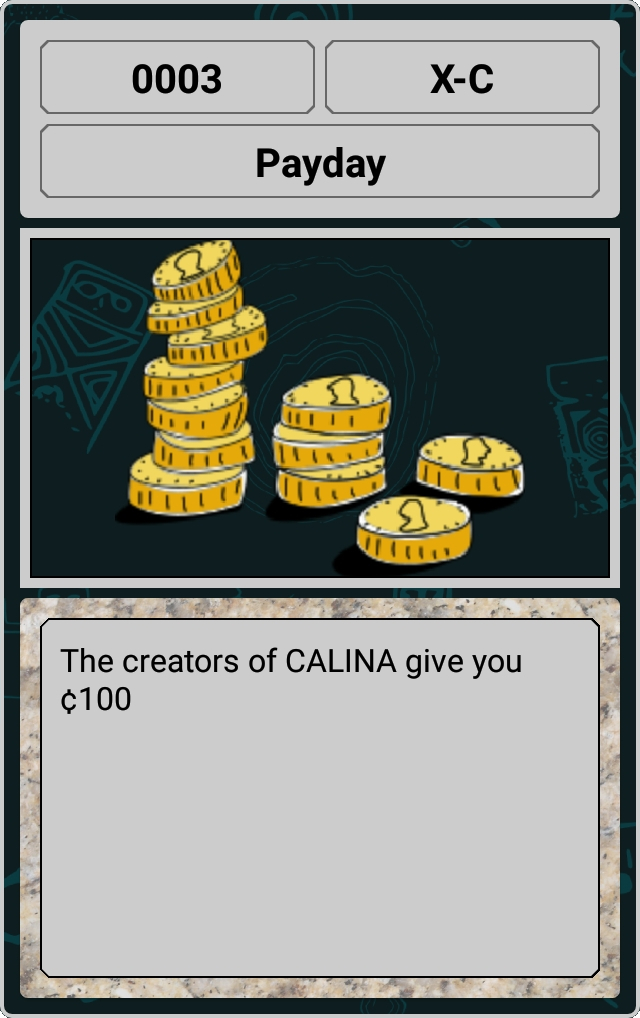
\includegraphics{screenshots/cartaacciondetalle}
	\end{adjustbox}
}
\\
{\footnotesize Fuente: de elaboración propia}
\end{figure}

Identificadas con la letra \textbf{X}, las cartas de acción son las mas versátiles de todos los tipos de 
cartas, y su función es la de mediar una intención que puede afectar situaciones en la vida real, por ejemplo 
subir una nota en particular una décima, ayudas en un examen, o lo que desee el profesor, con su 
correspondiente validación para confirmar la acción, por otro lado pueden afectar otras cartas mediante 
acciones pre-programadas en triggers adjuntos a la carta.

\section{Dificultad de obtención de las cartas}
\label{sec:app_dificultad}

Cada carta tiene asociado un nivel de dificultad para conseguir la carta, este valor es dado al momento de 
creación de la carta otorgado por el docente, según su criterio o diseño pedagógico, los posibles valores son
las letras 'C', 'B', 'A', 'S', 'SS' y 'X', estos símbolos representan los siguientes niveles de dificultad:

\begin{itemize}
	\item \textbf{(C)} Muy fácil
	\item \textbf{(B)} Fácil
	\item \textbf{(A)} Normal
	\item \textbf{(S)} Difícil
	\item \textbf{(SS)} Muy difícil
	\item \textbf{(X)} Únicas
\end{itemize}

\section{Crear un grupo}

\begin{figure}[!htb]
\caption[]{Aplicación CALINA, Secuencia para crear un grupo}
\centering
\begin{adjustbox}{width=15cm}
\begin{tikzpicture}
	\node[inner sep=0pt] (crear_grupo) at (0cm,0cm) {
\includegraphics[width=2cm]{screenshots/crear_grupo}};
	\node[inner sep=0pt] (dialogo_crear_grupo) at (2.5cm,0cm) {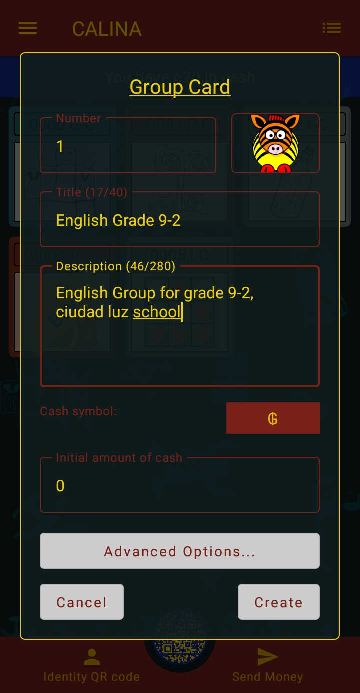
\includegraphics[width=2cm]{screenshots/dialogo_crear_grupo}};
	\node[inner sep=0pt] (grupo_creado) at (5cm,0cm) {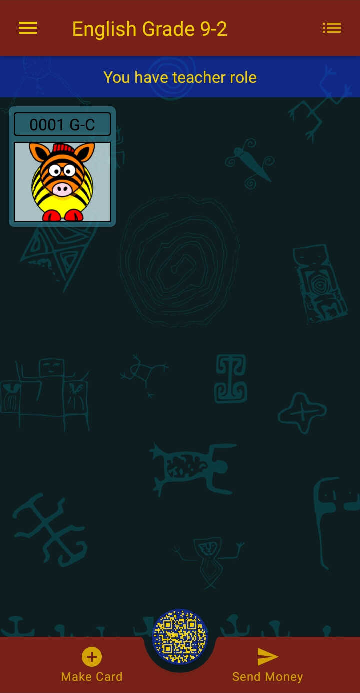
\includegraphics[width=2cm]{screenshots/grupo_creado}};
	\draw[-triangle 90] (crear_grupo) edge (dialogo_crear_grupo);
	\draw[-triangle 90] (dialogo_crear_grupo) edge (grupo_creado);
	\draw[red] (-1.5cm,-2.1cm) rectangle (6.3cm,2.3cm);
	\node[red, anchor=west] at (-1.2cm, 2cm) {\footnotesize Docente};
\end{tikzpicture}
\end{adjustbox}
\\
{\footnotesize Fuente: de elaboración propia}
\end{figure}

Inicialmente todos los usuarios de CALINA pertenecen al grupo (clase) bajo el mismo nombre CALINA, dependiendo 
del rol que decidas tomar puedes requerir crear un grupo para que tus estudiantes se suscriban en el caso que 
seas un profesor, o solamente inscribirse a un grupo creado previamente si eres estudiante.

Para crear un grupo en el caso que seas docente, debes seleccionar la opción de crear grupo en el menú de 
navegación. A continuación de muestra un diálogo para la creación de carta de grupo. En el cual se debe 
asignar un número de grupo con un valor entre 0 y 9999, un titulo para identificar el grupo de máximo 40
caracteres, y una descripción de máximo 280 caracteres para dar contexto al grupo que se esta creando.

También, se puede asignar un símbolo para la moneda virtual que va a manejar el grupo, esta moneda hace la
función de puntos de experiencia dentro de la estrategia de gamificación, y un valor inicial de efectivo con
la que todos los estudiantes van a iniciar al momento de suscribirse.

Adicional, se pueden asignar triggers a la tarjeta de grupo en opciones avanzadas, para ver la sintaxis en la 
creación de triggers dirigirse a la sección \ref{sec:app_triggers}.

Una vez creado el grupo, este es seleccionado y cambia el contexto de la aplicación asignando el rol de 
docentes, por lo que ya podemos crear cartas y compartir la suscripción al grupo.

\section{Suscribirse a un grupo}

\begin{figure}[!htb]
\caption[]{Aplicación CALINA, Secuencia para suscribirse a un grupo}
\centering
\begin{adjustbox}{width=15cm}
\begin{tikzpicture}
	\node[inner sep=0pt] (detail) at (0cm,0cm) {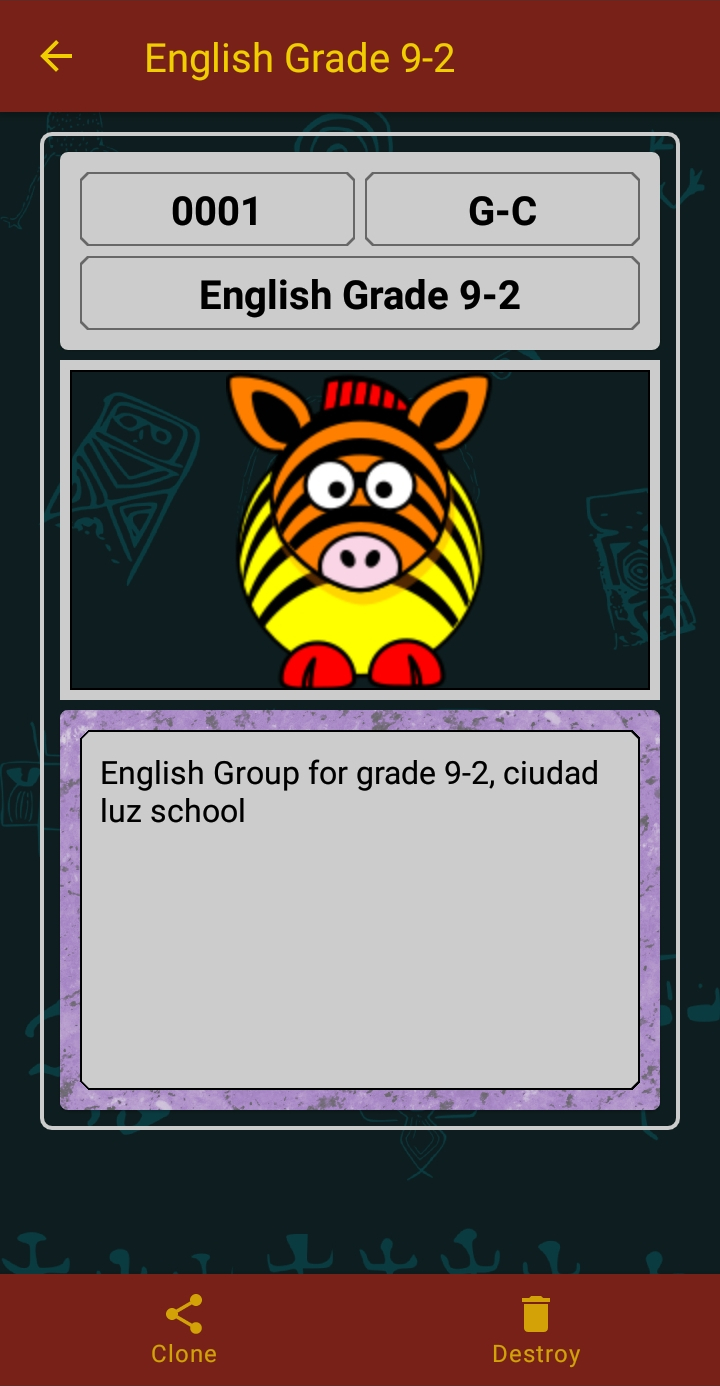
\includegraphics[width=2cm]{screenshots/detalle_grupo}};
	\node[inner sep=0pt] (clone) at (2cm,0cm) {
\includegraphics[width=0.8cm]{screenshots/clone}};
	\node[inner sep=0pt] (qrsuscripcion) at (4cm,0cm) {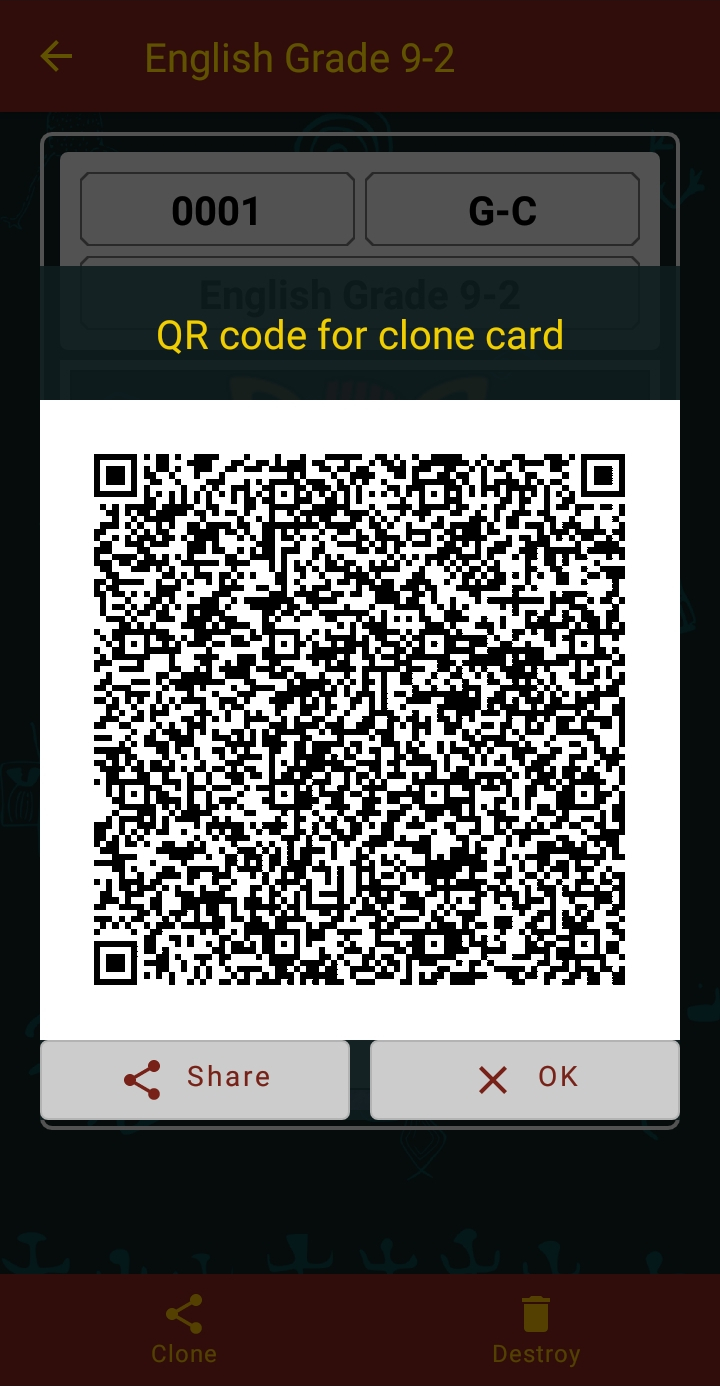
\includegraphics[width=2cm]{screenshots/qr_suscripcion}};
	\node[inner sep=0pt] (lectorQR) at (2cm,-4.5cm) {
\includegraphics[width=0.8cm]{screenshots/lectorQR}};
	\node[inner sep=0pt] (lector_qr) at (4cm,-4.5cm) {
\includegraphics[width=2cm]{screenshots/lector_qr}};
	\node[inner sep=0pt] (inscripcion_grupo) at (7cm,-4.5cm) {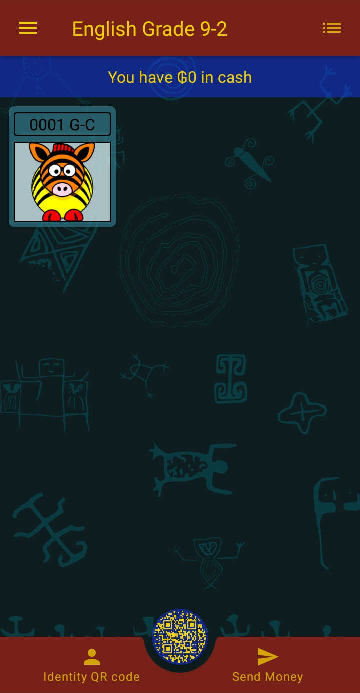
\includegraphics[width=2cm]{screenshots/inscripcion_grupo}};
	\draw[-triangle 90] (detail) edge (clone);
	\draw[-triangle 90] (clone) edge (qrsuscripcion);
	\draw[-triangle 90] (lectorQR) edge (lector_qr);
	\draw[-triangle 90] (qrsuscripcion) edge (lector_qr);
	\draw[-triangle 90] (lector_qr) edge (inscripcion_grupo);
	\draw[red] (-1.5cm,-2.1cm) rectangle (8.5cm,3cm);
	\draw[blue] (-1.5cm,-6.7cm) rectangle (8.5cm,-2.2cm);
	\node[red, anchor=west] at (-1.2cm, 2.4cm) {\footnotesize Docente};
	\node[blue, anchor=west] at (-1.2cm, -6cm) {\footnotesize Estudiante};
\end{tikzpicture}
\end{adjustbox}
\\
{\footnotesize Fuente: de elaboración propia}
\end{figure}

Una vez creado el grupo, el docente puede generar el código de suscripción para que sea leído o enviado a sus 
estudiantes, e ingresen al contexto gamificado de su clase. Por lo que se debe entrar al detalle de la tarjeta 
de grupo y pulsar la opción de clonar, una vez echo esto se genera un código QR que puede ser leído por el 
estudiante o enviado a través de medios digitales al usar la opción de compartir.

Una vez generado el código QR para la suscripción a un grupo, el estudiante puede leer este código usando el 
lector de códigos QR que trae incluida la aplicación, el cual se encuentra en el centro de la zona de 
controles, una vez leído el código la aplicación del estudiante ya se encuentra inscrito en el grupo bajo el 
contexto de estudiante, pudiendo ver en su contexto la tarjeta de grupo y el dinero virtual que posee.

Para des-suscribirse a un grupo al que ya no deseemos pertenecer, es tan sencillo como borrar (destruir) la 
tarjeta del grupo del que se desee salir, esta acción también borra las tarjetas asociadas al grupo eliminado.

\section{Código QR de identidad}

Siempre que se tenga el contexto de estudiante, se puede generar un código QR de identidad necesario para 
realizar transacciones como el envío de dinero o recibir cartas de regalo.

Este código funciona como un documento de identidad único para cada estudiante, y es la forma como CALINA 
garantiza las transacciones entre dos personas.

\begin{figure}[!htb]
\caption[]{Aplicación CALINA, secuencia generación código QR de identidad - Rol estudiante}
\centering
\begin{adjustbox}{width=9cm}
\begin{tikzpicture}
	\node[inner sep=0pt] (identity_button) at (0cm,0cm) {
\includegraphics[width=2cm]{screenshots/identity_button}};
	\node[inner sep=0pt] (identity_code) at (2.5cm,0cm) {
\includegraphics[width=2cm]{screenshots/identity_code}};
	\draw[-triangle 90] (identity_button) edge (identity_code);
	\draw[blue] (-1.5cm,-2.1cm) rectangle (4cm,2.3cm);
	\node[blue, anchor=west] at (-1.2cm, 2cm) {\footnotesize Estudiante};
\end{tikzpicture}
\end{adjustbox}
\\
{\footnotesize Fuente: de elaboración propia}
\end{figure}

\section{Acciones sobre las cartas}

Una vez dentro de un contexto, el estudiante puede acceder por diversas vías nuevas cartas las cuales puede 
usar dentro del desarrollo gamificado del curso, por lo que como cualquier objeto puede recibirlas, 
regalarlas, venderlas o intercambiarlas, según su conveniencia, y si son cartas de acción usarlas según vea 
necesario.

\subsection{Regalar cartas}
\label{sec:app_enviarcartas}

\begin{figure}[!htb]
\caption[]{Aplicación CALINA, Secuencia para regalar una carta}
\centering
\begin{adjustbox}{width=15cm}
\begin{tikzpicture}
	\node[inner sep=0pt] (gift)  at (2.5cm,1.5cm) {
\includegraphics[width=0.8cm]{screenshots/gift}};
	\node[inner sep=0pt] (advertencia) at (2.5cm,0cm) {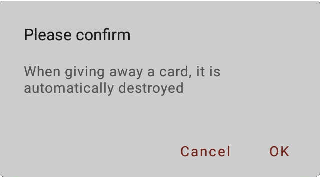
\includegraphics[width=2.5cm]{screenshots/advertencia}};
	\node[inner sep=0pt] (lectorQRID) at (5cm,0cm) {
\includegraphics[width=1.5cm]{screenshots/lector_qr}};
	\node[inner sep=0pt] (IDbutton)  at (2.5cm,-3.5cm) {
\includegraphics[width=1.5cm]{screenshots/identity_button}};
	\node[inner sep=0pt] (QRID) at (5cm,-3.5cm) {
\includegraphics[width=1.5cm]{screenshots/identity_code}};
	\node[inner sep=0pt] (QRgift) at (8cm,0cm) {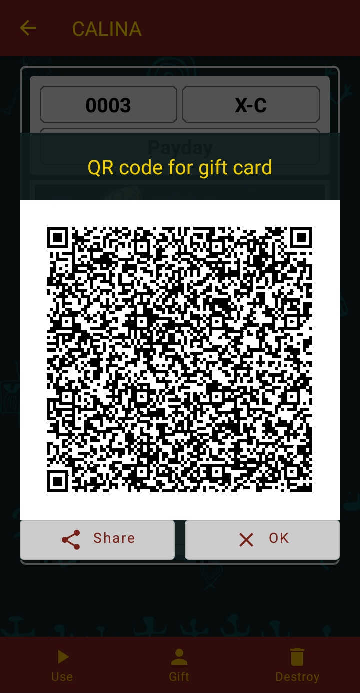
\includegraphics[width=1.5cm]{screenshots/QRgift}};
	\node[inner sep=0pt] (lectorQR) at (6.5cm,-3.5cm) {
\includegraphics[width=0.6cm]{screenshots/lectorQR}};
	\node[inner sep=0pt] (lectorQRgift) at (8cm,-3.5cm) {
\includegraphics[width=1.5cm]{screenshots/lector_qr}};
	\draw[-triangle 90] (gift) edge (advertencia);
	\draw[-triangle 90] (advertencia) edge (lectorQRID);
	\draw[-triangle 90] (IDbutton) edge (QRID);
	\draw[-triangle 90] (QRID) edge (lectorQRID);
	\draw[-triangle 90] (lectorQRID) edge (QRgift);
	\draw[-triangle 90] (lectorQR) edge (lectorQRgift);
	\draw[-triangle 90] (QRgift) edge (lectorQRgift);
	\draw[red] (1cm,-1.7cm) rectangle (9cm,2.8cm);
	\draw[blue] (1cm,-5.3cm) rectangle (9cm,-1.8cm);
	\node[red, anchor=west] at (1.3cm, 2.4cm) {\scriptsize Emisor};
	\node[blue, anchor=west] at (1.3cm, -4.8cm) {\scriptsize Receptor};
\end{tikzpicture}
\end{adjustbox}
\\
{\footnotesize Fuente: de elaboración propia}
\end{figure}

No todas las cartas se pueden obsequiar, eso depende de como es creada por parte del docente, sin embargo,
sera la opción mas común o por defecto, para regalar una carta por parte del docente o estudiante, se debe 
entrar en el detalle de la carta que se desee obsequiar, y dar un toque a la opción ``regalar'', esto ocasiona 
que salga una advertencia ya que la carta va a ser borrada del estudiante que va a obsequiar la tarjeta, al 
confirmar esta advertencia se solicita leer un código QR con la identidad del estudiante a quien va dirigido 
el regalo, una vez leído este código se genera el código QR de transferencia.

Finalmente, este código debe ser leído por el estudiante a quien va dirigida la carta, ocasionando que se 
genere la tarjeta en la aplicación del estudiante receptor.

\subsection{Comercio o intercambio de cartas entre estudiantes}

En CALINA se pueden vender o intercambiar tarjetas, sin embargo no hay necesidad de tener controles 
adicionales para realizar dichas acciones, ya que el vender o el intercambiar objetos implica un contrato 
social de buena voluntad entre dos personas, por lo que al regalar y al mismo tiempo recibir tarjetas con 
una persona implica un trueque, o al enviar una carta y recibir dinero de la otra persona que esta recibiendo 
la tarjeta implica una venta. Para realizar estas acciones se debe enviar tarjetas, visto en la sección 
\ref{sec:app_enviarcartas} y enviar dinero en la sección \ref{sec:app_enviardinero}.

\subsection{Clonar cartas - Docente}

\begin{figure}[!htb]
\caption[]{Aplicación CALINA, secuencia clonación de cartas para enviar a estudiantes}
\centering
\begin{adjustbox}{width=9cm}
\begin{tikzpicture}
	\node[inner sep=0pt] (clone) at (0cm,0cm) {
\includegraphics[width=0.8cm]{screenshots/clone}};
	\node[inner sep=0pt] (QRclone) at (2.5cm,0cm) {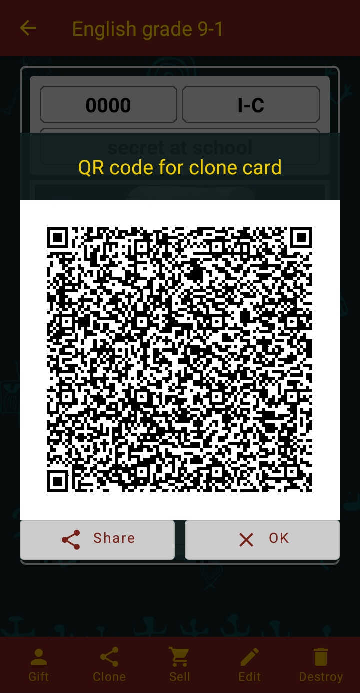
\includegraphics[width=2cm]{screenshots/QRclone}};
	\draw[-triangle 90] (clone) edge (QRclone);
	\draw[red] (-1.5cm,-2.1cm) rectangle (4cm,2.3cm);
	\node[red, anchor=west] at (-1.2cm, 2cm) {\footnotesize Docente};
\end{tikzpicture}
\end{adjustbox}
\\
{\footnotesize Fuente: de elaboración propia}
\end{figure}

Esta es la forma más habitual que tiene el docente de enviar tarjeta a los estudiantes, tiene la misma función 
de regalar una carta, con la diferencia, que al realizar clonar no se va a borrar la carta del conjunto de 
cartas del docente y adicionalmente no se solicita el QR de identidad del estudiante que recibe la carta, por 
lo que este código puede ser leído por cualquier estudiante que tenga la capacidad de leerlo. Por ejemplo, se 
puede imprimir para que los estudiantes simplemente lean el código y la carta sea transmitida.

\subsection{Cartas para la venta - Docente}

\begin{figure}[!htb]
\caption[]{Aplicación CALINA, secuencia creación de cartas para la venta a estudiantes}
\centering
\begin{adjustbox}{width=15cm}
\begin{tikzpicture}
	\node[inner sep=0pt] (sell) at (0cm,0cm) {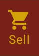
\includegraphics[width=0.8cm]{screenshots/sell}};
	\node[inner sep=0pt] (cantidad_venta) at (2.5cm,0cm) {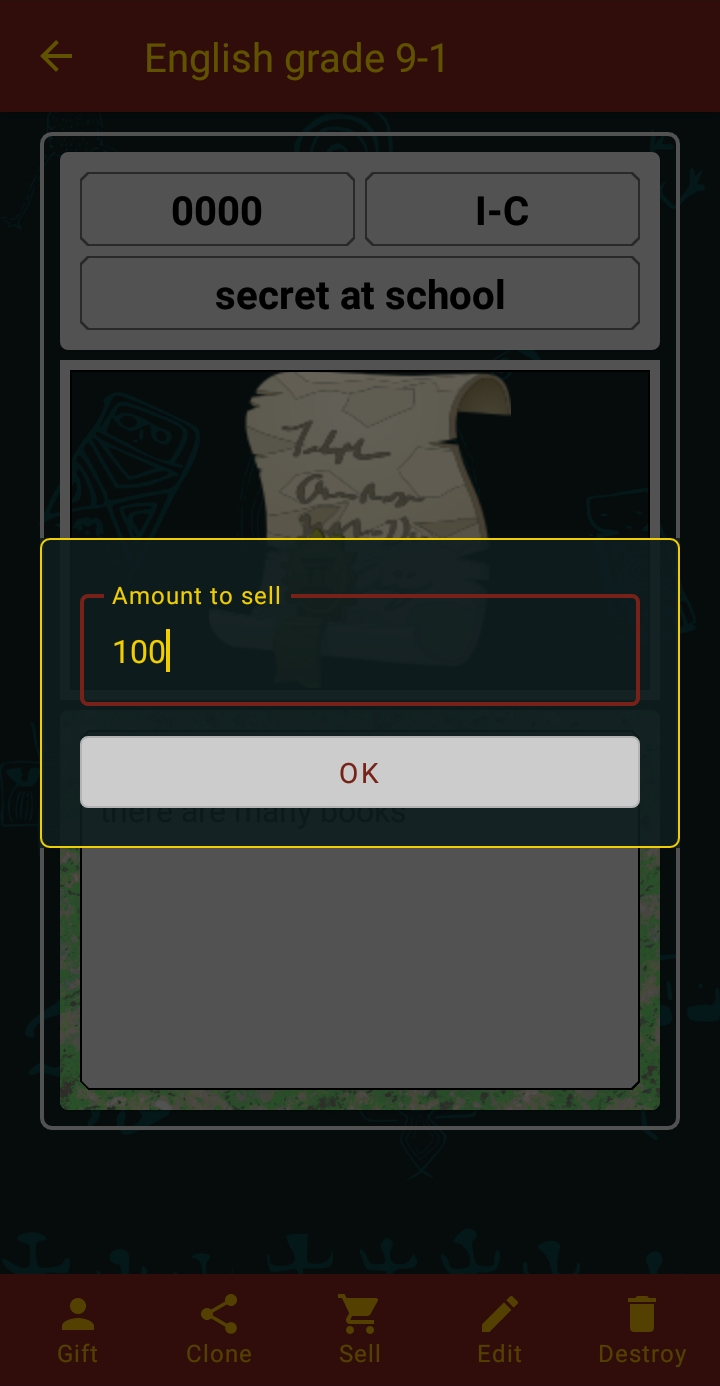
\includegraphics[width=2cm]{screenshots/cantidad_venta}};
	\node[inner sep=0pt] (QRventa) at (5cm,0cm) {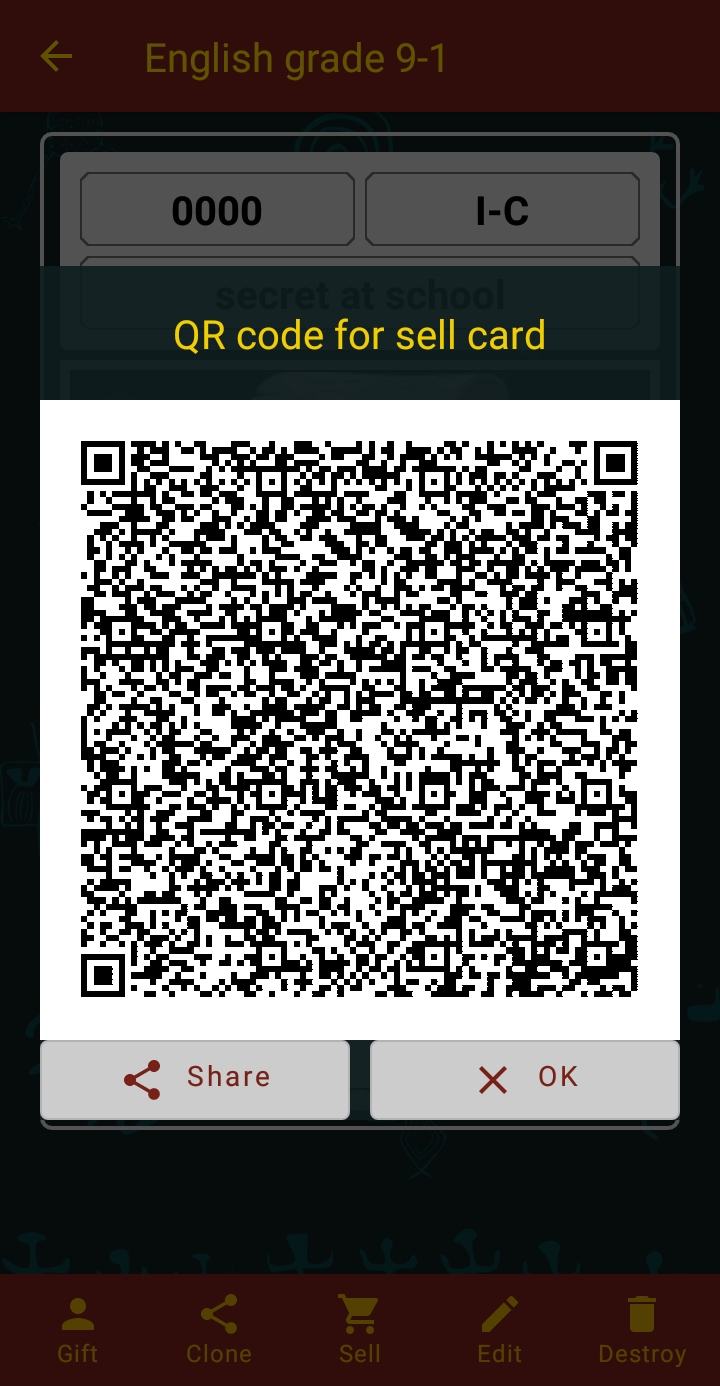
\includegraphics[width=2cm]{screenshots/QRventa}};
	\draw[-triangle 90] (sell) edge (cantidad_venta);
	\draw[-triangle 90] (cantidad_venta) edge (QRventa);
	\draw[red] (-1.5cm,-2.1cm) rectangle (6.5cm,2.3cm);
	\node[red, anchor=west] at (-1.2cm, 2cm) {\footnotesize Docente};
\end{tikzpicture}
\end{adjustbox}
\\
{\footnotesize Fuente: de elaboración propia}
\end{figure}

El proceso es similar a clonar cartas, con la diferencia que se pregunta antes de generar el código de 
transferencia por un monto de dinero para poder usar o desbloquear la tarjeta por parte del estudiante. De 
esta manera podemos generar un conjunto de tarjetas desbloqueables con los puntos de experiencia (dinero 
virtual) para publicar vía virtual o impresa y motivar a los estudiantes en su progreso.

\subsection{Comprar una carta - Estudiante}

\begin{figure}[!htb]
\caption[]{Aplicación CALINA, secuencia compra de cartas por el estudiante}
\centering
\begin{adjustbox}{width=15cm}
\begin{tikzpicture}
	\node[inner sep=0pt] (minibuy) at (0cm,0cm) {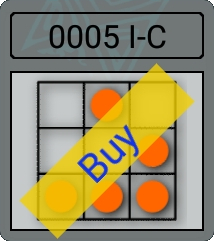
\includegraphics[width=0.8cm]{screenshots/minibuy}};
	\node[inner sep=0pt] (cardbuy) at (2cm,0cm) {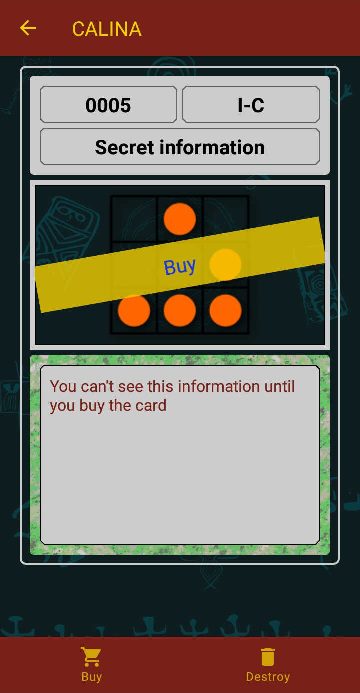
\includegraphics[width=2cm]{screenshots/cardbuy}};
	\node[inner sep=0pt] (buy) at (4cm,0cm) {
\includegraphics[width=0.5cm]{screenshots/buy}};
	\node[inner sep=0pt] (dialogbuy) at (6cm,0cm) {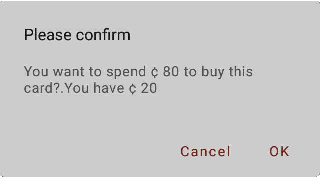
\includegraphics[width=2.5cm]{screenshots/dialogbuy}};
	\node[inner sep=0pt] (nomoney) at (9cm,0cm) {
\includegraphics[width=2.5cm]{screenshots/nomoney}};
	\node[inner sep=0pt] (cardbuy2) at (6cm,-3cm) {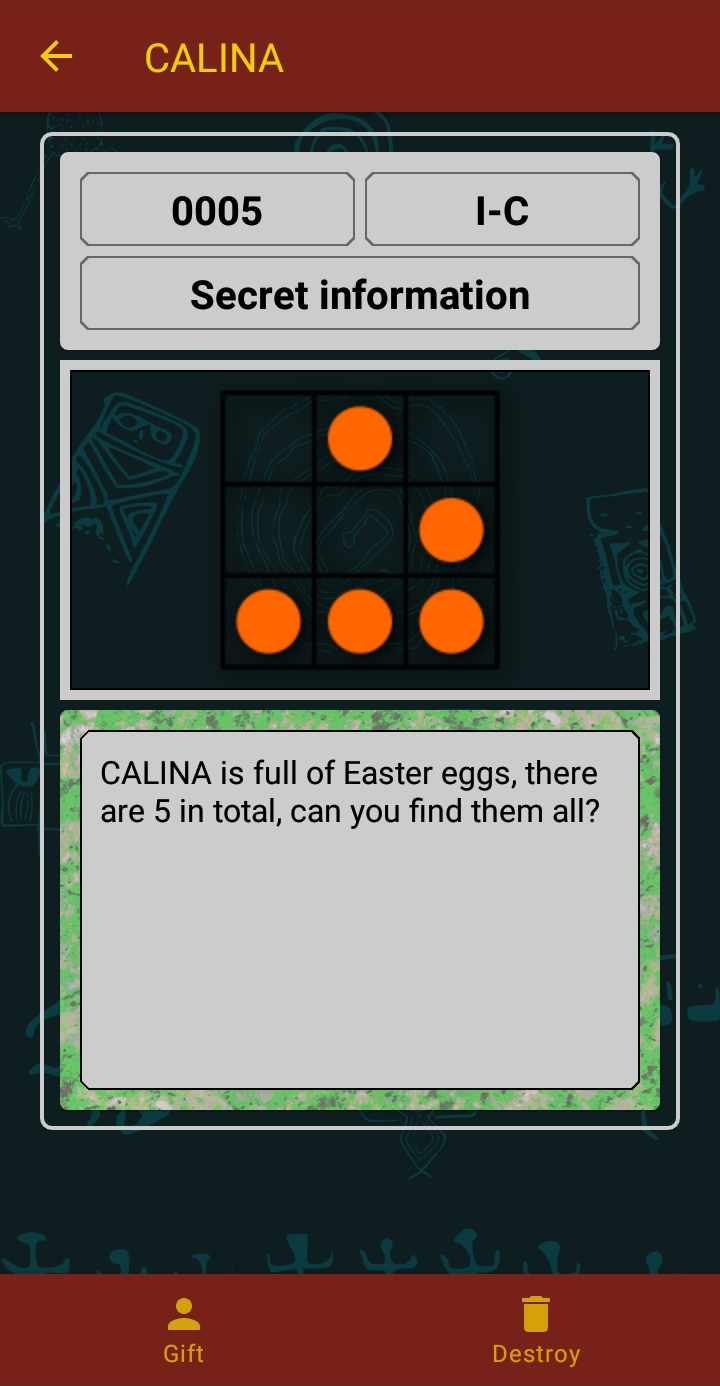
\includegraphics[width=2cm]{screenshots/cardbuy2}};
	\draw[-triangle 90] (minibuy) edge (cardbuy);
	\draw[-triangle 90] (cardbuy) edge (buy);
	\draw[-triangle 90] (buy) edge (dialogbuy);
	\draw[-triangle 90] (dialogbuy) edge (nomoney);
	\draw[-triangle 90] (dialogbuy) edge (cardbuy2);
	\draw[blue] (-0.7cm,-5.3cm) rectangle (10.5cm,3cm);
	\node[blue, anchor=west] at (0cm, 2.5cm) {\footnotesize Estudiante};
\end{tikzpicture}
\end{adjustbox}
\\
{\footnotesize Fuente: de elaboración propia}
\end{figure}

Cuando se recibe una carta para la compra por parte del estudiante, su tarjeta aparece con una etiqueta que 
indica que la carta debe ser comprada, esta etiqueta aparece tanto en el listado de cartas como en el detalle 
de la carta en si, por lo que para usarla en el caso de las cartas de acción se debe desbloquear comprándola, 
en el caso de las cartas de información no se podrá leer la descripción que esta contenga, en el caso de las 
cartas trofeo y de grupo, no se poseerá la recompensa ni se pertenecerá al grupo en cuestión hasta que sean 
compradas.

Para la compra de cartas, se debe tener el dinero suficiente para la compra, de lo contrario no se hará dicha 
compra dentro del contexto que se este. En caso de que se cuente con el dinero suficiente y se confirme la 
transacción, el dinero es descontado automáticamente y la carta queda en un estado normal para su uso.

\subsection{Usar (cartas de acción)}

\begin{figure}[!htb]
\caption[]{Aplicación CALINA, secuencia usar cartas por el estudiante}
\centering
\begin{adjustbox}{width=15cm}
\begin{tikzpicture}
	\node[inner sep=0pt] (use) at (0cm,0cm) {
\includegraphics[width=0.7cm]{screenshots/use}};
	\node[inner sep=0pt] (msguse) at (2cm,0cm) {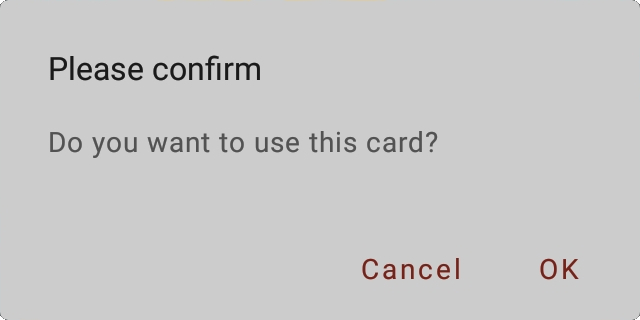
\includegraphics[width=2.5cm]{screenshots/msguse}};
	\node[inner sep=0pt] (name) at (4.8cm,0cm) {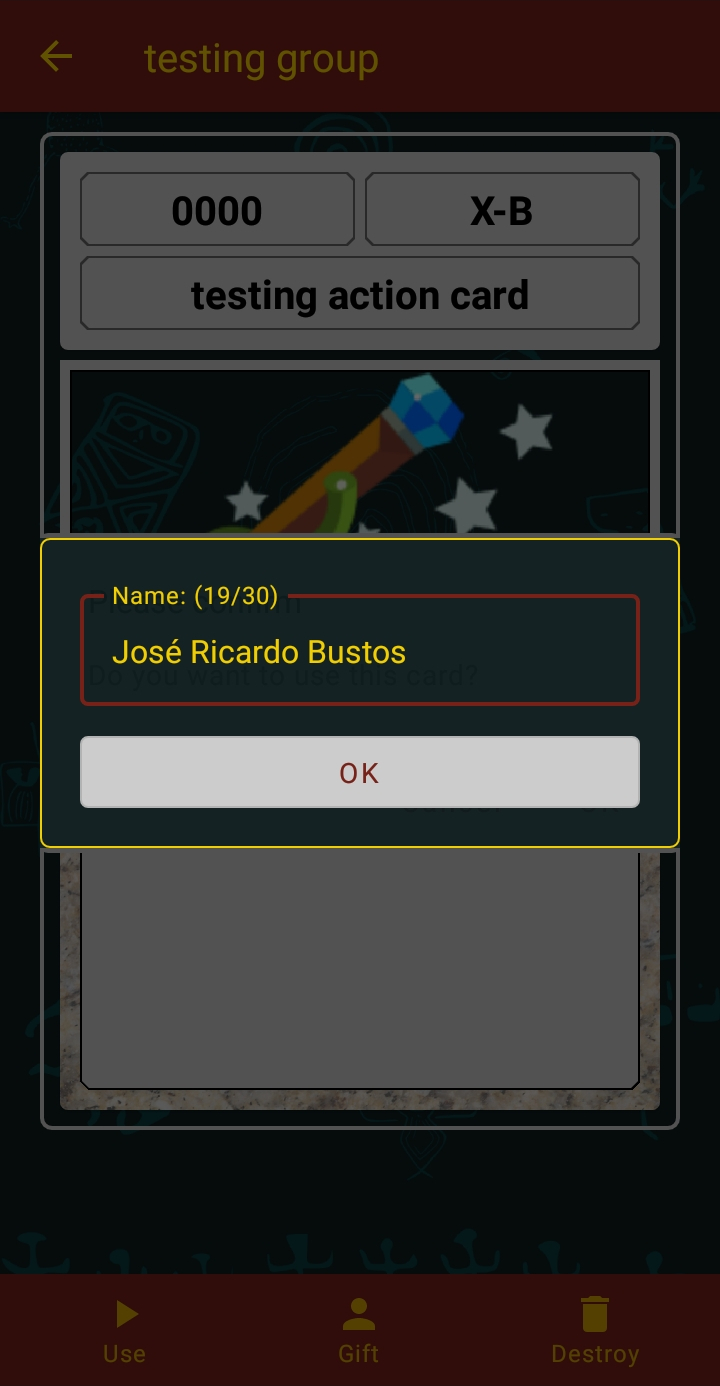
\includegraphics[width=2cm]{screenshots/name}};
	\node[inner sep=0pt] (used) at (7.3cm,0cm) {\includegraphics[width=2cm]{screenshots/used}};
	\node[inner sep=0pt] (usedmini) at (9cm,0cm) {\includegraphics[width=1cm]{screenshots/usedmini}};
	\draw[-triangle 90] (use) edge (msguse);
	\draw[-triangle 90] (msguse) edge (name);
	\draw[-triangle 90] (name) edge (used);
	\draw[blue] (-0.7cm,-2.3cm) rectangle (9.8cm,3cm);
	\node[blue, anchor=west] at (0cm, 2.5cm) {\footnotesize Estudiante};
\end{tikzpicture}
\end{adjustbox}
\\
{\footnotesize Fuente: de elaboración propia}
\end{figure}

Las cartas de acción en CALINA, son la base de la estrategia gamificada a usar en la clases, son las cartas 
que el estudiante puede usar para realizar un cambio en su desarrollo escolar, si este así lo desea, por 
ejemplo puede existir una carta que le brinde una mejora en sus calificaciones, ayuda en alguna pregunta de 
un examen, o lo que el docente considere. Para realizar la acción CALINA pregunta el nombre a quien se aplica 
esta acción y quedará registrado en la tarjeta para su posterior validación.

Aunque los \textit{triggers} pueden se pueden usar con todo tipo de cartas, las cartas de acción tienen un 
evento especial que se dispara cuando el usuario usa una carta, lo que se puede aprovechar también para 
afectar el entorno de la aplicación calina al ser usada una acción. Ver a la sección \ref{sec:app_triggers} 
para ver el listado de acciones habilitadas que existen.

\subsection{Validación de cartas - rol estudiantes}

\begin{figure}[!htb]
\caption[]{Aplicación CALINA, secuencia validación de cartas usadas}
\centering
\begin{adjustbox}{width=15cm}
\begin{tikzpicture}
	\node[inner sep=0pt] (validate0) at (-0.5cm,0cm) {\includegraphics[width=0.7cm]{screenshots/validate0}};
	\node[inner sep=0pt] (validate) at (1.5cm,0cm) {\includegraphics[width=2.5cm]{screenshots/validate}};
	\node[inner sep=0pt] (validate2) at (4.5cm,0cm) {\includegraphics[width=2.5cm]{screenshots/validate2}};
	\node[inner sep=0pt] (validate3) at (7.5cm,0cm) {\includegraphics[width=2.5cm]{screenshots/validate3}};
	\draw[-triangle 90] (validate0) edge (validate);
	\draw[-triangle 90] (validate) edge (validate2);
	\draw[-triangle 90] (validate2) edge (validate3);
	\draw[blue] (-1.8cm,-2.7cm) rectangle (9.1cm,3.3cm);
	\node[blue, anchor=west] at (-1.3cm, 2.9cm) {\footnotesize Estudiante};
\end{tikzpicture}
\end{adjustbox}
\\
{\footnotesize Fuente: de elaboración propia}
\end{figure}

Una vez usada una carta de acción que tiene consecuencias en la vida real, se aconseja que el estudiante 
realice el proceso de validación con el docente, esto es que el estudiante envíe de regreso al docente la 
carta usada que esta etiquetada con su nombre, para que el docente verifique su autenticidad y realice las 
acciones que lleven a lugar en el mundo real y que la carta de acción por lo tanto tenga consecuencias.

\subsection{Editar (cartas de información)}
\label{sec:app_edit}

\begin{figure}[!htb]
\caption[]{Aplicación CALINA, secuencia edición de cartas}
\centering
\begin{adjustbox}{width=15cm}
\begin{tikzpicture}
	\node[inner sep=0pt] (edit2) at (0cm,0cm) {\includegraphics[width=2.5cm]{screenshots/edit2}};
	\node[inner sep=0pt] (edit) at (2cm,0cm) {\includegraphics[width=0.7cm]{screenshots/edit}};
	\node[inner sep=0pt] (edit3) at (4cm,0cm) {\includegraphics[width=2.5cm]{screenshots/edit3}};
	\node[inner sep=0pt] (edit4) at (7.5cm,0cm) {\includegraphics[width=2.5cm]{screenshots/edit4}};
	\draw[-triangle 90] (edit2) edge (edit);
	\draw[-triangle 90] (edit) edge (edit3);
	\draw[-triangle 90] (edit3) edge (edit4);
	\draw[blue] (-1.8cm,-2.7cm) rectangle (9.1cm,3.3cm);
	\node[blue, anchor=west] at (-1.3cm, 2.9cm) {\footnotesize Estudiante};
\end{tikzpicture}
\end{adjustbox}
\\
{\footnotesize Fuente: de elaboración propia}
\end{figure}

Esta es una acción especial para cartas de tipo informativas, si el docente lo desea puede habilitar que una 
carta de información se pueda editar su descripción, esto con el fin de pasar mensajes entre personas del 
grupo, usarse para escritura colaborativa o creativa, o lo que desee el docente dentro de su planeación 
pedagógica, incluso juntar esta opción con triggers de la sección \ref{sec:app_triggers} y dar premios si se 
contesta adecuadamente una pregunta.

\subsection{Destruir cartas}

Esta opción solo esta disponible para cartas que no tengan fecha de caducidad o sean la carta del grupo 
inicial de CALINA, su función luego de preguntar si realmente se desea eliminar la carta es eliminarla por 
completo de la aplicación.

\section{Cartas con alcance global}
\label{sec:app_global}

Cuando se crean cartas estas pueden tener un alcance global, no solo local, esto quiere decir que pueden 
servir para cualquier grupo perteneciente al mismo creador (profesor), por lo que una carta global puede ser 
compartida a estudiantes de distintos grupos, o estudiantes de distintos cursos intercambiarlas.

\section{Fecha de expiración}
\label{sec:app_expired}

\begin{figure}[!htb]
\caption[]{Aplicación CALINA, mensaje de expiración en cartas}
\centering
\begin{adjustbox}{width=5cm}
\begin{tikzpicture}
	\node[inner sep=0pt] at (0cm,0cm) {\includegraphics[width=7cm]{screenshots/movil}};
	\node[inner sep=0pt] at (-0.05cm,0.05cm) {\includegraphics[width=5.95cm]{screenshots/expired}};
\end{tikzpicture}
\end{adjustbox}
\\
{\footnotesize Fuente: de elaboración propia}
\end{figure}

Para crear un sentimiento de presión de tiempo, un profesor puede crear cartas con fecha de caducidad, esto 
con el objetivo de ser usada o existir solo en un periodo de tiempo, este tipo de cartas no pueden ser 
eliminadas manualmente, y solo se borraran si se sale del grupo o si llega su fecha de expiración de forma 
automática. Por ejemplo, es útil si se quiere crear una carta que de puntos (dinero) por asistencia de clase 
publicarla a la entrada y que el estudiante solo pueda usarla una única vez, evitando trampas y cumpliendo con 
el objetivo de la carta en cuestión.

Al entrar al detalle de una carta aparece un mensaje indicando el número de días para ser eliminada o en caso 
contrario si esta no vence nunca.

\section{Divisas virtuales}
\label{sec:app_enviardinero}

\begin{figure}[!htb]
\caption[]{Aplicación CALINA, Secuencia para enviar dinero}
\centering
\begin{adjustbox}{width=15cm}
\begin{tikzpicture}
	\node[inner sep=0pt] (sendmoney)  at (1cm,0cm) {\includegraphics[width=1.2cm]{screenshots/sendmoney}};
	\node[inner sep=0pt] (sendmoney2) at (3cm,0cm) {\includegraphics[width=1.5cm]{screenshots/sendmoney2}};
	\node[inner sep=0pt] (lectorQRID) at (5cm,0cm) {\includegraphics[width=1.5cm]{screenshots/lector_qr}};
	\node[inner sep=0pt] (IDbutton)  at (3cm,-3.5cm) {\includegraphics[width=1.2cm]{screenshots/identity_button}};
	\node[inner sep=0pt] (QRID) at (5cm,-3.5cm) {\includegraphics[width=1.5cm]{screenshots/identity_code}};
	\node[inner sep=0pt] (sendmoney3) at (8cm,0cm) {\includegraphics[width=1.5cm]{screenshots/sendmoney3}};
	\node[inner sep=0pt] (lectorQR) at (6.5cm,-3.5cm) {\includegraphics[width=0.6cm]{screenshots/lectorQR}};
	\node[inner sep=0pt] (lectorQRgift) at (8cm,-3.5cm) {\includegraphics[width=1.5cm]{screenshots/lector_qr}};
	\node[inner sep=0pt] (sendmoney4) at (8cm,-7cm) {\includegraphics[width=1.2cm]{screenshots/sendmoney4}};
	\node[inner sep=0pt] (sendmoney5) at (6cm,-7cm) {\includegraphics[width=1.5cm]{screenshots/sendmoney5}};
	\node[inner sep=0pt] (use) at (4.5cm,-7cm) {\includegraphics[width=0.7cm]{screenshots/use}};
	\node[inner sep=0pt] (sendmoney6) at (3cm,-7cm) {\includegraphics[width=1.5cm]{screenshots/sendmoney6}};
	\node[inner sep=0pt] (sendmoney7) at (1cm,-7cm) {\includegraphics[width=1.2cm]{screenshots/sendmoney7}};
	\draw[-triangle 90] (sendmoney) edge (sendmoney2);
	\draw[-triangle 90] (sendmoney2) edge (lectorQRID);
	\draw[-triangle 90] (IDbutton) edge (QRID);
	\draw[-triangle 90] (QRID) edge (lectorQRID);
	\draw[-triangle 90] (lectorQRID) edge (sendmoney3);
	\draw[-triangle 90] (lectorQR) edge (lectorQRgift);
	\draw[-triangle 90] (QRgift) edge (lectorQRgift);
	\draw[-triangle 90] (lectorQRgift) edge (sendmoney4);
	\draw[-triangle 90] (sendmoney4) edge (sendmoney5);
	\draw[-triangle 90] (sendmoney5) edge (use);
	\draw[-triangle 90] (use) edge (sendmoney6);
	\draw[-triangle 90] (sendmoney6) edge (sendmoney7);
	\draw[red] (0cm,-1.7cm) rectangle (9cm,2.8cm);
	\draw[blue] (0cm,-9cm) rectangle (9cm,-1.8cm);
	\node[red, anchor=west] at (0.3cm, 2.4cm) {\scriptsize Emisor};
	\node[blue, anchor=west] at (0.3cm, -2.3cm) {\scriptsize Receptor};
\end{tikzpicture}
\end{adjustbox}
\\
{\footnotesize Fuente: de elaboración propia}
\end{figure}

Esta es la principal forma que tiene CALINA para asignar puntos de experiencia dentro de la estrategia 
gamificada, aunque su uso no es obligatorio ya que todo depende del diseño del docente y sus intenciones, por 
regla cada grupo tiene su propio contexto por lo tanto su propia moneda (a pesar que puedan manejar el mismo 
símbolo).

El estudiante puede recibir dinero virtual de dos maneras: a través de transferencias directas de dinero por 
parte del profesor o un compañero que este en el mismo grupo, o por intercambio de cartas sobre todo de tipo 
acción que tengan un \textit{trigger} que añada dinero a la cuenta del estudiante, esto se ve en la sección 
\ref{sec:app_triggers} y se usa sobretodo si se desea crear una carta que de dinero y se pueda clonar, como el 
caso de tarjetas para dar puntos por asistencia. Para el caso de transferencia directa de dinero, siempre se 
requiere la lectura del código de identificación del estudiante que va a recibir el dinero, para 
posteriormente generar una carta de acción con el número ``7777'' que puede ser usada para añadir el dinero, 
esta tarjeta también puede ser regalada posteriormente por el estudiante, sin embargo, la tarjeta tiene fecha 
de caducidad de un día para su uso, tiempo de cual se desaparece.

\section{Esquema de niveles}

El desarrollo de niveles de experiencia para los estudiantes, esta diseñado en la aplicación CALINA, sin 
embargo esta pendiente de desarrollo para una versión futura.

\section{Creación de cartas desde el rol de profesor}
\label{sec:app_creacioncartas}

\begin{figure}[H]
\caption[]{Aplicación CALINA, creación de cartas rol de profesor}
\centering
\subfloat[Botón para crear cartas]{
	\begin{adjustbox}{width=1.5cm}
		\includegraphics{screenshots/create}
	\end{adjustbox}
}
\hspace{1cm}
\subfloat[Selección tipo de carta a crear]{
	\begin{adjustbox}{width=5cm}
	\begin{tikzpicture}
		\node[inner sep=0pt] at (0cm,0cm) {\includegraphics[width=7cm]{screenshots/movil}};
		\node[inner sep=0pt] at (-0.05cm,0.05cm) {\includegraphics[width=5.95cm]{screenshots/create2}};
	\end{tikzpicture}
	\end{adjustbox}
}
\hspace{1cm}
\subfloat[Diálogo de creación de carta]{
	\begin{adjustbox}{width=5cm}
	\begin{tikzpicture}
		\node[inner sep=0pt] at (0cm,0cm) {\includegraphics[width=7cm]{screenshots/movil}};
		\node[inner sep=0pt] at (-0.05cm,0.05cm) {\includegraphics[width=5.95cm]{screenshots/create3}};
	\end{tikzpicture}
	\end{adjustbox}
}
\\
{\footnotesize Fuente: de elaboración propia}
\end{figure}

La creación de cartas es el trabajo más importante que debe realizar el profesor, si se trabaja con CALINA 
para la mediación de su estrategia gamificada, por lo tanto es el docente el qué debe definir que cartas 
crear, cómo serán dadas a los estudiantes, cómo va a ser la asignación de puntos, etc. Es importante anotar 
nuevamente que CALINA solo es una herramienta que media para el uso de gamificación, mas no es una herramienta 
mágica que de per se va a motivar a sus estudiantes a lograr sus metas, por lo tanto, es la estrategia 
pedagógica diseñada y desarrolla concienzudamente por el docente la que logra esto.

CALINA permite crear cartas si se tiene asignado el rol de docente, esto es, si se creo un grupo desde la 
aplicación, por lo que cualquiera puede crear sus cartas, pero estas solo se pueden usar con las personas que 
se suscriban al grupo que se crea para esto, por lo que cartas de otros docentes no pueden ser usadas en un 
contexto particular.

Continuando, el proceso de crear una carta es relativamente sencillo, sin embargo a continuación se aclara 
cada uno de los elementos que pueden personalizarse:

\begin{description}
  \item[Número] \hfill \\ Es un número que permite identificar la tarjeta por parte del docente, si se desea 
	  no necesariamente es un número único, su valor debe estar entre 0 y 9999.
  \item[Imagen] \hfill \\ La selección de imagen genera un diálogo nuevo que se trata mas adelante en esta 
	  misma sección.
  \item[Título] \hfill \\ Un título de no más de 40 caracteres que permite al igual que el número a 
	  identificar una tarjeta.
  \item[Descripción] \hfill \\ Una descripción para darle contexto a la carta que se esta creando, permitiendo 
	  a los estudiantes conocer su función o su intención, no puede tener más de 280 caracteres.
  \item[Dificultad] \hfill \\ La dificultad se trata en la sección \ref{sec:app_dificultad}, es el nivel de 
	  dificultad que considera el docente tiene el estudiante de conseguir esta carta.
  \item[Regalable] \hfill \\ Se marca si se desea que el estudiante tenga la opción de regalarlo a otros 
	  compañeros, si se deja deshabilitado el estudiante que reciba la tarjeta no podrá intercambiarlo con 
	  otros compañeros, solamente borrarlo.
  \item[Clonable] \hfill \\ Se marca si se desea que el docente pueda hacer clonaciones de la carta o crear 
	  cartas de ventas.
  \item[Global] \hfill \\ El alcance de la carta se trata en la sección \ref{sec:app_global}, se marca si se 
	  desea que la carta este habilitada para todos los grupos creados por el docente.
  \item[Editable] \hfill \\ Esta opción solo sale para cartas de tipo informativas, este tema se trata en la 
	  sección\ref{sec:app_edit}.
  \item[Opciones avanzadas] \hfill \\ Las opciones avanzadas, tiene dos elementos adicionales para potenciar 
	  el uso de las cartas creadas en CALINA, las fechas de expiración tratadas en la sección 
	  \ref{sec:app_expired} y los \textit{triggers} que se tratan en la sección \ref{sec:app_triggers}.
\end{description}

\vspace{1em}

\begin{figure}[!htb]
\caption[]{Aplicación CALINA, creación de cartas opciones avanzadas}
\centering
\subfloat[Diálogo opciones avanzadas]{
	\begin{adjustbox}{width=4cm}
	\begin{tikzpicture}
		\node[inner sep=0pt] at (0cm,0cm) {\includegraphics[width=7cm]{screenshots/movil}};
		\node[inner sep=0pt] at (-0.05cm,0.05cm) {\includegraphics[width=5.95cm]{screenshots/create4}};
	\end{tikzpicture}
	\end{adjustbox}
}
\hspace{1cm}
\subfloat[Carta con fecha de expiración]{
	\begin{adjustbox}{width=4cm}
	\begin{tikzpicture}
		\node[inner sep=0pt] at (0cm,0cm) {\includegraphics[width=7cm]{screenshots/movil}};
		\node[inner sep=0pt] at (-0.05cm,0.05cm) {\includegraphics[width=5.95cm]{screenshots/create5}};
	\end{tikzpicture}
	\end{adjustbox}
}
\hspace{1cm}
\subfloat[Diálogo de selección de fecha]{
	\begin{adjustbox}{width=4cm}
	\begin{tikzpicture}
		\node[inner sep=0pt] at (0cm,0cm) {\includegraphics[width=7cm]{screenshots/movil}};
		\node[inner sep=0pt] at (-0.05cm,0.05cm) {\includegraphics[width=5.95cm]{screenshots/create6}};
	\end{tikzpicture}
	\end{adjustbox}
}
\\
{\footnotesize Fuente: de elaboración propia}
\end{figure}

La selección de una imagen para la carta le permite dar contexto a la carta, e incluso inspirar sentimientos 
en los estudiantes, por lo que es de gran importancia, calina cuenta con 34 símbolos y 404 imágenes para 
seleccionar, tome el tiempo en seleccionar la imagen para que tenga relación con la descripción y título de 
la carta que se esta creando, incluso relación con otras cartas que se hayan creado previamente.

\begin{figure}[!htb]
\caption[]{Aplicación CALINA, selección de imagen para carta}
\centering
\begin{adjustbox}{width=4.5cm}
\begin{tikzpicture}
	\node[inner sep=0pt] at (0cm,0cm) {\includegraphics[width=7cm]{screenshots/movil}};
	\node[inner sep=0pt] at (-0.05cm,0.05cm) {\includegraphics[width=5.95cm]{screenshots/selectimg}};
\end{tikzpicture}
\end{adjustbox}
\\
{\footnotesize Fuente: de elaboración propia}
\end{figure}

\section{Especificación de \textit{triggers}}
\label{sec:app_triggers}

Los \textit{triggers} son fragmentos de código ejecutables que cada una de las tarjetas puede contener 
almacenado, estas son acciones que se ejecutan de forma automática al presentarse un evento, y al momento que 
se cumpla una condición ejecute una consecuencia, que puede afectar la propia carta o incluso cartas del mismo 
grupo. El objetivo de los \textit{triggers} es potenciar las posibilidades de acciones de las cartas, y 
enriquecer el contexto propio de las tarjetas. Por ejemplo, con los \textit{triggers} se puede hacer un 
contador que cada vez que se lea un tarjeta de información aumente su valor, y al llegar a 10 muestre 
información adicional, este es solo un ejemplo, la posibilidad de combinación de eventos + condiciones + 
consecuencias potencia el uso de CALINA de forma significativa.

La especificación de \textit{triggers} se va a realizar en lenguaje formal de expresiones regulares 
(\textbf{regex}),

\theoremstyle{definition}
\newtheorem{definition}{Definición}[section]

\begin{definition}[\textit{triggers}]
	{\Large\color{blue}\verb/^((/}{\Large\color{red}\verb/T/}{\Large\color{blue}\verb/|)*/}
	{\Large\color{red}\verb/T/}{\Large\color{blue}\verb/)?$/}\ donde {\Large\color{red}\verb/T/}\ es la 
	definición de una sentencia de un \textit{trigger} especifico que es definido a continuación, esto es 
	por que una carta puede tener varios \textit{triggers} separados por el símbolo 
	{\Large\color{blue}\verb/|/}.
\end{definition}

\begin{definition}[\textcolor{red}{T} (\textit{trigger})]
	{\Large\color{red} \verb/E/}{\Large\color{blue} \verb/_/}{\Large\color{red} \verb/C/}{\Large\color{blue} \verb/(#/}{\Large\color{red} \verb/C/}{\Large\color{blue} \verb/)*/}{\Large\color{blue} \verb/_/}{\Large\color{red} \verb/A/}{\Large\color{blue} \verb/(#/}{\Large\color{red} \verb/A/}{\Large\color{blue} \verb/)*/}
	donde {\Large\color{red}\verb/E/}\ es la especificación de un evento, {\Large\color{red} \verb/C/}{\Large\color{blue} \verb/(#/}{\Large\color{red} \verb/C/}{\Large\color{blue} \verb/)*/}
	es la especificación de las condiciones que pueden ser varias separadas por el símbolo 
	{\Large\color{blue}\verb/#/}, y {\Large\color{red} \verb/A/}{\Large\color{blue} \verb/(#/}{\Large\color{red} \verb/A/}{\Large\color{blue} \verb/)*/} 
	es la especificación de las consecuencias las cuales pueden ser varias separadas por el símbolo 
	{\Large\color{blue}\verb/#/}, todas separadas por el símbolo {\Large\color{blue}\verb/_/}.
\end{definition}

\begin{definition}[\textcolor{red}{E} (Evento)]
	{\Large\color{blue} \verb/[UGRDBEVWLXSZ]/}
	un evento esta descrito por una única letra, y especifica en que momento el \textit{trigger} se 
	ejecuta, los posibles valores son:

	\begin{itemize}
		\item {\Large\color{blue} \verb/U/}: Sucede cuando una carta de acción es usada
		\item {\Large\color{blue} \verb/G/}: Sucede cuando una carta es regalada, efectos como cambio 
			de título, descripción, estado, imagen, etc., no aplican para este evento, debido a 
			que se envía la carta sin aplicar cambios, para realizar cambios en la carta se deben 
			hacer en el evento de recibir
		\item {\Large\color{blue} \verb/R/}: Sucede cuando una carta es recibida
		\item {\Large\color{blue} \verb/D/}: Sucede cuando una carta es destruida
		\item {\Large\color{blue} \verb/B/}: Sucede cuando una carta es comprada
		\item {\Large\color{blue} \verb/E/}: Sucede cuando una carta de información es editada
		\item {\Large\color{blue} \verb/V/}: Sucede cuando una carta de acción es validada, efectos 
			como cambio de título, descripción, estado, imagen, etc., no aplican para este evento, 
			debido a que se envía la carta sin aplicar cambios que llega al docente
		\item {\Large\color{blue} \verb/W/}: Sucede cuando una carta es abierta y se muestra su detalle
		\item {\Large\color{blue} \verb/L/}: Sucede cuando una carta es listada
		\item {\Large\color{blue} \verb/X/}: Sucede cuando una carta es eliminada por vencimiento de fecha
		\item {\Large\color{blue} \verb/S/}: Sucede cuando una carta de grupo es seleccionada
	\end{itemize}
\end{definition}

\begin{definition}[\textcolor{red}{C} (Condición)]
	{\Large\color{blue} \verb/[TRCDNISEWMLXHA](:[^|_#:]+)*/}
	Una condición esta descrita por una única letra inicial, y un grupo de parámetros separados por el 
	carácter {\Large\color{blue} \verb/:/}, el número de parámetros puede ser cero si no se requieren y 
	esto depende del tipo de condición que se desea usar:

	\begin{itemize}
		\item {\Large\color{blue} \verb/T/}: Verdadero siempre, no tiene condición (parámetros = 0)
		\item {\Large\color{blue} \verb/R:[0-9]{1,3}/}: Verdadero al azar con una probabilidad entre 0 y 
			99.9\% (parámetros = 1)
		\item {\Large\color{blue} \verb/C:[0-9]+/}: Verdadero cuando el contador llega al valor que 
			indica el parámetro (parámetros = 1)
		\item {\Large\color{blue} \verb/D:[0-9]+/}: Verdadero cuando han pasado ``x'' días desde el día 
			de creación de la carta (parámetros = 1)
		\item {\Large\color{blue} \verb/N(:[0-9]+)+/}: Verdadero cuando la carta esta acompañada por las 
			cartas numeradas en los parámetros (parámetros >= 1)
		\item {\Large\color{blue} \verb/I:[0-9]+/}: Verdadero cuando la carta pertenece al usuario que 
			tiene el identificador registrado en el parámetro (parámetros = 1)
		\item {\Large\color{blue} \verb/S:[NUB]/}: Verdadero cuando la carta tiene el estado que 
			indica  el parámetro, los posibles estados son normal (N), usada (U) y en proceso de 
			compra (B) (parámetros = 1)
		\item {\Large\color{blue} \verb/E:[0-9]+/}: Verdadero cuando faltan ``x'' días para el día 
			de vencimiento de la carta (parámetros = 1)
		\item {\Large\color{blue} \verb/W:[^|_#:]+/}: Verdadero cuando la carta tiene en la descripción 
			exactamente el texto que indica el parámetro, se usa en cartas de tipo información que 
			se pueda editar (parámetros = 1)
		\item {\Large\color{blue} \verb/M:[0-9]+/}: Verdadero cuando en el contexto se tiene más de 
			``x'' cantidad de dinero (parámetros = 1)
		\item {\Large\color{blue} \verb/X:[0-9]+/}: Verdadero cuando en el contexto se tiene más de 
			``x'' cantidad de cartas (parámetros = 1)
		\item {\Large\color{blue} \verb/L:[^|_#:]+/}: Verdadero cuando en el contexto se tiene el valor
			del nivel que describe el parámetro (Por implementar, parámetros = 1)
		\item {\Large\color{blue} \verb/H:[1-3]?[0-9]:1?[0-9]:[0-9][0-9][0-9][0-9]/}: Verdadero cuando 
			en se está en la fecha que indica los parámetros (parámetros = 3)
		\item {\Large\color{blue} \verb/A:[0-9]+/}: Verdadero cuando han pasado ``x'' días desde el 
			registro de fecha (parámetros = 1)
	\end{itemize}
\end{definition}

\begin{definition}[\textcolor{red}{A} (Consecuencia)]
	{\Large\color{blue} \verb/[DMCTYINXZREUHGVQAB](:[^|_#:]+)*/}
	Una consecuencia esta descrita por una única letra inicial, y un grupo de parámetros separados por el 
	carácter {\Large\color{blue} \verb/:/}, el número de parámetros puede ser cero si no se requieren y 
	esto depende del tipo de consecuencia que se desea usar:

	\begin{itemize}
		\item {\Large\color{blue} \verb/D/}: Borra la tarjeta (parámetros = 0)
		\item {\Large\color{blue} \verb/M:-?[0-9]+/}: Resta o adiciona dinero del contexto actual de 
			acuerdo al parámetro (parámetros = 1)
		\item {\small\color{blue} \verb/C:[^|_#:]{1,40}:[^|_#:]{1,280}:[XIRG]:[CBASWX]:[0-9]{1,4}:[^|_#:]+:[10]/}: 
			Crea una carta nueva con el título como \uline{primer} parámetro, la descripción como 
			\uline{segundo} parámetro, en \uline{tercer} lugar el tipo de carta 
			{\Large\color{blue} \verb/X/} para carta de acción, {\Large\color{blue} \verb/I/} para 
			informativa, {\Large\color{blue} \verb/R/} para de tipo recompensa, y 
			{\Large\color{blue} \verb/G/} para carta de tipo agrupación, un \uline{cuarto} 
			parámetro para la dificultad de la carta, {\Large\color{blue} \verb/C/} para muy fácil,
			{\Large\color{blue} \verb/B/} para fácil, {\Large\color{blue} \verb/A/} para normal,
			{\Large\color{blue} \verb/S/} para difícil, {\Large\color{blue} \verb/W/} para muy 
			difícil, {\Large\color{blue} \verb/X/} para de tipo única, un \uline{quinto} parámetro 
			para indicar el número de la tarjeta, un \uline{sexto} parámetro para la imagen 
			asignada a la carta que puede ser item1-item404 o symbol1-symbol34 para un total de 
			438 imágenes disponibles, y por último un \uline{séptimo} parámetro para indicar si se 
			puede intercambiar al tener un 1 asignado (parámetros = 7)
		\item {\Large\color{blue} \verb/T:[^|_#:]{1,40}/}: Modifica el título de la carta con el valor del 
			parámetro (parámetros = 1)
		\item {\Large\color{blue} \verb/Y:[CBASWX]/}: Modifica la dificultad de la carta con el valor 
			dado por el parámetro, {\Large\color{blue} \verb/C/} para muy fácil, 
			{\Large\color{blue} \verb/B/} para fácil, {\Large\color{blue} \verb/A/} para normal, 
			{\Large\color{blue} \verb/S/} para difícil, {\Large\color{blue} \verb/W/} para muy 
			difícil, {\Large\color{blue} \verb/X/} para de tipo única (parámetros = 1)
		\item {\Large\color{blue} \verb/I:[^|_#:]+/}: Modifica la imagen de la carta con el valor del 
			parámetro puede ser item1-item404 o symbol1-symbol34 para un total de 438 imágenes 
			disponibles (parámetros = 1)
		\item {\Large\color{blue} \verb/N:[^|_#:]{1,280}/}: Modifica la descripción de la carta con el 
			valor del parámetro (parámetros = 1)
		\item {\Large\color{blue} \verb/X/}: Aumenta en uno un contador (parámetros = 0)
		\item {\Large\color{blue} \verb/Z/}: Disminuye en uno un contador (parámetros = 0)
		\item {\Large\color{blue} \verb/R/}: Pone el contador en cero (parámetros = 0)
		\item {\Large\color{blue} \verb/E/}: Hace que una carta informativa sea editable si no lo es, 
			o deje de serlo si es editable (parámetros = 0)
		\item {\Large\color{blue} \verb/U/}: Hace que una carta de acción que tenga el estado de usada 
			se pueda a volver a usar (parámetros = 0)
		\item {\Large\color{blue} \verb/H/}: Puede clonar cualquier carta del conjunto de cartas 
			(menos la de tipo grupo) al azar (parámetros = 0)
		\item {\Large\color{blue} \verb/G:[^|_#:]{1,280}/}: Muestra un Mensaje informando al estudiante
			(parámetros = 1)
		\item {\Large\color{blue} \verb/V/}: Borra todos los trigger de la tarjeta (parámetros = 0)
		\item {\Large\color{blue} \verb/Q/}: Cambia el imei de la tarjeta (parámetros = 0)
		\item {\Large\color{blue} \verb/A/}: Hace un registro de fecha (parámetros = 0)
		\item {\Large\color{blue} \verb/B/}: Borra el registro de fecha (parámetros = 0)
	\end{itemize}

\end{definition}

\subsection{Ejemplos de triggers comunes o útiles}

\begin{itemize}
	\item {\Large\color{blue} \verb/U_T_M:100/}: Adiciona 100 de dinero virtual cuando una carta de acción 
		es usada, este \textit{trigger} es útil para crear cartas que den puntos por asistencia, al 
		crear una carta de acción con fecha de caducidad y añadiendo este \textit{trigger}.
	\item {\Large\color{blue} \verb/E_W:RESPUESTA_M:100#E#G:Respuesta Correcta/}: Adiciona 100 de dinero 
		virtual cuando un estudiante edita una carta de información, y pone la RESPUESTA en algún 
		lugar de la descripción, adicional hace que la carta ya no sea editable y muestra un mensaje 
		con la frase ``Respuesta Correcta''.
	\item {\Large\color{blue} \verb/Z_T_X|Z_C:5_M:100#R/}: Adiciona 100 de dinero virtual cada vez que 
		ingresa el estudiante 5 veces al grupo.
	\item {\Large\color{blue} \verb/R_R:010_Y:X/}: Modifica la dificultad de una carta a única, con una
		probabilidad del 1\% al momento de ser recibida.
	\item {\Large\color{blue} \verb/V_T_M:100/}: Adiciona 100 de dinero virtual cuando una carta es 
		validada con el docente.
	\item {\Large\color{blue} \verb/U_T_I:item64/}: Al ser usada una carta de acción esta modifica su 
		imagen y ahora muestra un dragón acuático.
	\item {\Large\color{blue} \verb/D_T_C:FANTASMA:CARTA FANTASMA:R:S:666:item210:0/}: Al ser borrada la
		carta, se crea una carta de recompensa con el título de ``FANTASMA'', de dificultad difícil, 
		con el número de identificación 666, la imagen de un fantasma, la cual no puede ser 
		intercambiada.
	\item {\Large\color{blue} \verb/R_T_A|L_A:2_X#A/}: Cada 2 días la carta de acción se habilita 
		pudiendo usarla de nuevo.
	\item {\Large\color{blue} \verb/U_R:200_M:100/}: Una carta de acción que tiene el 20\% de probabilidad 
		de darme 100 de dinero virtual al ser usada.
	\item {\Large\color{blue} \verb/U_T_H/}: Al ser usada una carta de acción, puede clonar al azar a 
		cualquier tarjeta que este en el inventario (menos las de tipo grupo).
	\item {\normalsize\color{blue} \verb/G_N:666_C:DIAMANTE ARCOÍRIS:RARA PIEDRA PRECIOSA:R:W:888:item311:1/}: 
		Al ser regalada la carta, si el estudiante tiene además la carta número 666, se crea la carta
		número 888 de nombre ``DIAMANTE ARCOÍRIS'' de tipo recompensa que se puede intercambiar.
\end{itemize}

%\section{Misión de entrenamiento}
%
%En la instalación inicial de CALINA los estudiantes van a pertenecer inicialmente al grupo CALINA, por lo que
%es la única tarjeta que van a poseer, esto se hace con el propósito de no saturar a los educandos con tarjetas 
%que aún no saben su propósito, uso o razón. Así el docente que vaya trabajar con ellos puede implementar su 
%propia misión de entrenamiento, y la misión inicial de CALINA no se robe el protagonismo.
%
%[IMAGEN]
%
%La misión inicial de CALINA va a hacer uso extensivo, de la estrategia de carrera de observación y los huevos 
%de pascua. Para esto la carta de agrupación cuenta con un botón de enlace externo hacia un documento alojado 
%en \textit{google drive}, el cual contiene un manual reducido de CALINA y las primeras cartas para adquirir 
%por medio de un catalogo
%
%[CARTAS DEL CATALOGO]
%
%Sin embargo estas no son las únicas cartas, para mostrar las posibilidades que tiene CALINA se hace uso 
%extensivo de los \textit{triggers}, a continuación se muestran las cartas adicionales y como se pueden 
%obtener,
%
%[CARTAS ADICIONALES]
%
%\section{Estrategias gamificadas con CALINA}
%
%Normalmente el uso de cartas de CALINA ya de por si es suficientemente enriquecedor en la aplicación de 
%estrategias gamificadas en nuestra clase, sin embargo, CALINA puede ser de ayuda bajo otros contextos, 
%complementando el uso de otras estrategias que los docentes puede usar, a continuación se mencionan algunos 
%ejemplos que se pueden usar.
%
%\subsection{Puntos por asistencia}
%
%LOREM
%
%\subsection{Catalogo de cartas a la venta}
%
%LOREM
%
%\subsection{Carrera de observación}
%
%LOREM
%
%\subsection{\textit{Scape room}}
%
%LOREM
%
%\subsection{\textit{Trivia}}
%
%LOREM
%
%\subsection{Desafíos}
%
%LOREM
%
%\subsection{Reforzamiento conductual con CALINA}
%
%LOREM
%
%\subsection{Narración de historias (\textit{Story telling})}
%
%LOREM
%
%\subsection{Juegos de rol (\textit{RPG})}
%
%LOREM
%
%\subsection{Huevos de pascua}
%
%LOREM
%
